\chapter{\textit{CP} parameter measurement}

The measurement of $\it{CP}$ parameters $\mathcal{S}$ and $\mathcal{A}$ is perform by fitting  Equation \ref{eq:tdcpv_sig} to the distribution of the decay time difference $\Delta t$ of events with flavor $q$, where $\Delta t = t_{CP}-t_{tag}$ and $q =  +1~(-1)$ when the tag-side $B$ meson is $B^0$~($\bar{B^0}$). 
\begin{equation}\label{eq:tdcpv_sig}
\mathcal{P}_{sig}(\Delta t, q ) = 
\frac{e^{-|\Delta t|/\tau_{B^0}}}{4\tau_{B^0}}
\begin{Bmatrix}
1 + q \cdot 
\begin{bmatrix}
\mathcal{S}\cdot\text{sin}(\Delta M_d \Delta t) + 
\mathcal{A}\cdot\text{cos}(\Delta M_d \Delta t)
\end{bmatrix}
\end{Bmatrix}
\end{equation}

The Equation \ref{eq:tdcpv_sig} describes the distribution of signal events only with $\tau_{B^0}$ and $\Delta M_d$ as physics parameters. To perform the unbinned maximum likelihood fit on data, a complete model for \textit{i}-th event that takes into account background and outlier components is defined as:
\begin{equation}\label{eq:tdcpv_all}
\begin{split}
\mathcal{P}(\Delta t_i,q_i,f^{sig}_i,\mathcal{S},\mathcal{A})
&=(1-f_{ol})\begin{bmatrix}f^{sig}_i\mathcal{P}_{sig}(\Delta t_i,q_i,\mathcal{S},\mathcal{A})+(1-f^{sig}_i)\mathcal{P}_{bkg}(\Delta t_i)
\end{bmatrix}\\
&+f_{ol}\mathcal{P}_{ol}(\Delta t_i)~,
\end{split}
\end{equation}
where $f^{sig}_i$ is the signal fraction assigned to the $i$-th event and $f_{ol}$ is the fraction of the outlier components, respectively. The $\mathcal{P}_{bkg}$ and $\mathcal{P}_{ol}$ are defined as
\begin{equation}\label{eq:p_bkg}
\mathcal{P}_{bkg} (\Delta t_i)=
f_{bkg}^{\delta}\delta(\Delta t_i-\mu_{bkg}^{\delta})+(1-f_{bkg}^{\delta})
\frac{1}{2\tau_{bkg}}e^{-|\Delta t_i-\mu_{\tau}^{bkg}|/\tau_{bkg}}~,
\end{equation}
\begin{equation}\label{eq:p_out}
\mathcal{P}_{ol} (\Delta t_i)=
G(\Delta t_i, \sigma_{ol})~,
\end{equation}
where $\delta(\Delta t_i-\mu_{bkg}^{\delta})$ is a Dirac $\delta$ function and $G$ is a single Gaussian. The outlier component is to improve the fit quality with large $\Delta t$ events. 

\section{Vertex Resolution Model}

The Equation \ref{eq:tdcpv_all} presents an ideal distribution of $\Delta t_i$ for each event without considering the difference between measured and the true position of the vertex. The difference can be described by introducing resolution functions, turning Equation \ref{eq:tdcpv_all} into Equation \ref{eq:tdcpv_all_res}.
\begin{equation}\label{eq:tdcpv_all_res}
\begin{split}
\mathcal{P}(\Delta t_i,q_i,f_i^{sig},\mathcal{S},\mathcal{A})
&=(1-f_{ol})\text{[}f^{sig}_i\mathcal{P}_{sig}(\Delta t_i)\otimes R_{sig}(\Delta t_i)\\
&+(1-f^{sig}_i)\mathcal{P}_{bkg}(\Delta t_i)\otimes R_{bkg}(\Delta t_i)
\text{]}\\
&+f_{ol}\mathcal{P}_{ol}(\Delta t_i)\otimes R_{ol}(\Delta t_i)
\end{split}
\end{equation}

The $R_{sig}$ stands for the resolution function for signal events, which receives smearing effect from \textit{CP}-side and tag-side separately, namely $R_{cp}$ and  $R_{tag}$. The treatment of \textit{CP}-side and tag-side is different because of the different vertexing strategies. For \textit{CP} side, the vertex of $B^0$ is reconstructed by fitting all the daughter particles using \textit{TreeFit}. Instead, in tag-side, there is no full reconstruction of $B^0$ so that a vertex fit is applied for the selected charged tracks in the Rest-Of-Event using \textit{KFit}. The background events have its own resolution model which is independent from  $\it{CP}$ violation parameters. The outlier component is used to smooth fit for large $\Delta t$ events. In the low statistics case like the current luminosity, the outlier component is not taken into account in the fit model of Equation \ref{eq:tdcpv_all_res}.

For signal events, the resolution functions are studied for $\it{CP}$-side and tag-side based on each possible degradation such as detector resolutions, the effect of tracks from non-primary $B$ vertex and so on. Such approaches have been used in Belle analyses. Details are summarized in Ref.~\cite{Yusa-note}. The vertex position difference $\Delta z$ for signal events can be broken down to 
\begin{equation}\label{eq:dz}
\Delta z 
=\Delta z^{'} + (z_{cp}^{}- z_{cp}^{'}) - (z_{tag}^{}- z_{tag}^{'}) ~,
\end{equation}
where the primed ones stand for physics truth of the position and the non-primed one are the measured value. Importantly, the resolution functions on both $\it{CP}$- and tag-sides depend on the applied IP constraints since it will change the obtained information of vertices. Considering that the fine structure of IP profile is not yet fully understood and small discrepancies have been observed between data and simulation~\cite{jpsiks_ichep}, there is no IP constraint applied for both sides in vertex fit to avoid the potential bias from  IP profile under this low statistical situation. From the Equation \ref{eq:dz}, the total vertex resolution of signal events can be presented as the sum of the two variables which stand for the resolution effects on the both sides. Therefore, the vertex resolution function of signal events is defined as
\begin{equation}\label{eq:Rsig}
R_{sig}=R_{cp}\otimes R_{tag}
\end{equation}
where $R_{cp}$ and $R_{tag}$ are the vertex resolution functions for $\it{CP}$-side and tag-side, respectively. 
The determination of these two components are described in Section 5.1.1 and 5.1.2.
\subsection{$\it{CP}$-side resolution function}
A $\it{CP}$-side vertex position is obtained by \textit{TreeFit} with all tracks from a reconstructed $B^0$, thus the resolution models only depend on the performance of the Belle II detectors, such as the vertexing and tracking accuracy affected by the detector hardware and software. Hence, the resolution effects for each event can be different based on event-by-event reconstruction quality, primarily presented by the reduced $\chi^2$ called $\chi^2/N$ from \textit{TreeFit}, which $N$ is the degree of freedom of the fit. The distribution of $\chi^2/N$ in data are shown in Figure \ref{fig:redchi2} compared with that of \textit{generic MC}. The error bar is taken as $\sqrt{N}$ where $N$ is the number of events in each bin.

\begin{figure}[htpb]
	\centering
	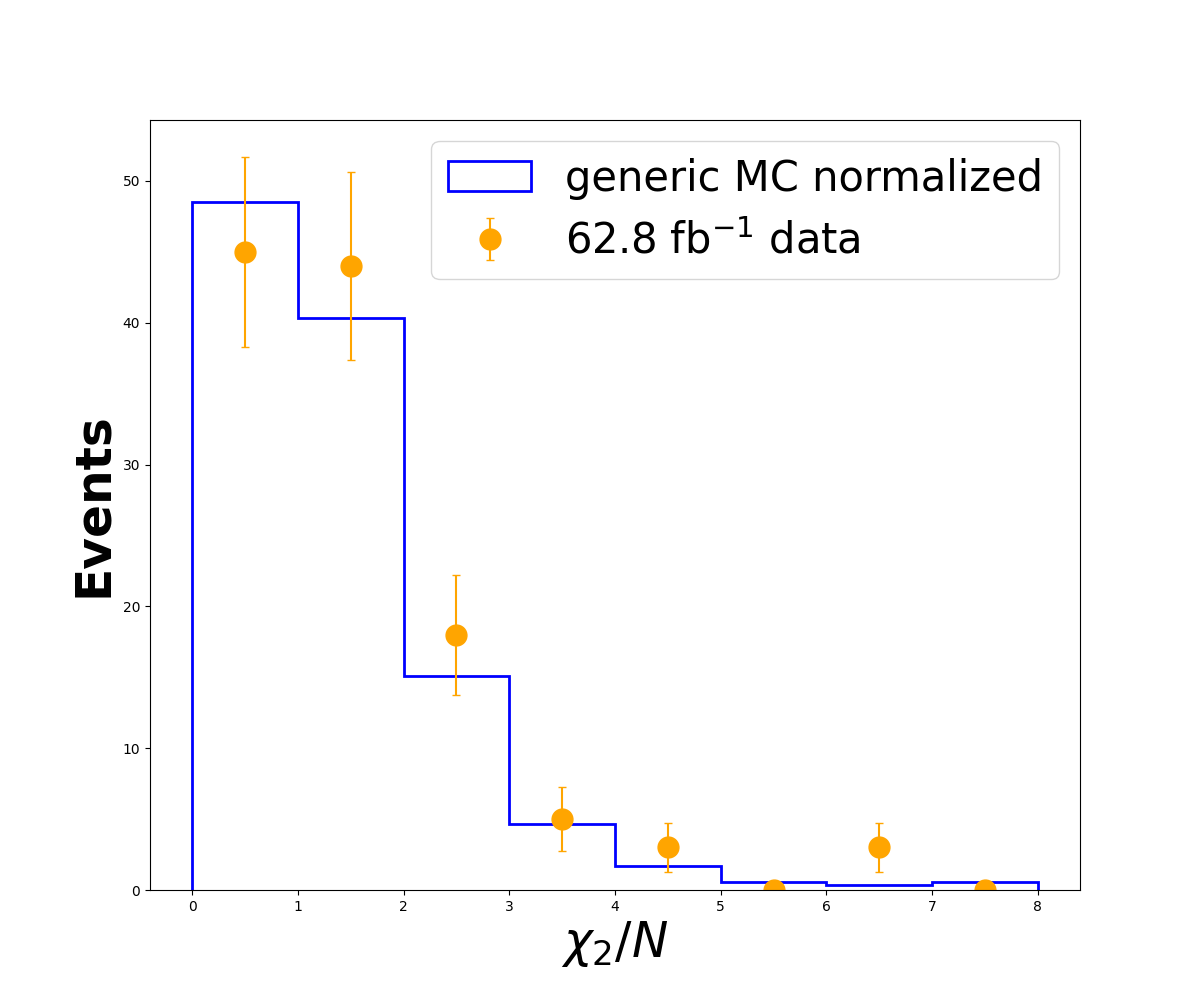
\includegraphics[height=6cm]{2D_redChi2.png}
	\caption{The distirbution of $\chi^2/N$ in selected events from data compared with that of \textit{generic MC}.}
	\label{fig:redchi2}
\end{figure}

We model the resolution function $R_{cp}$ on $\it{CP}$-side by using a double Gaussian function, where the mean is fixed to zero and the standard deviation is the error of reconstructed vertex $\sigma_{z_{cp}}$ scaled by $\chi^2/N$:
\begin{equation}\label{eq:Rcp}
R_{cp}(\delta z_{cp}) = (1-f_{cp}^{tail})G(0,s_{cp}^{main})+
f_{cp}^{tail}G(0,s_{cp}^{tail})~,
\end{equation}
where $s_{cp}^{main}$ and $s_{cp}^{tail}$ are
\begin{eqnarray}\label{eq:scp_mt}
\begin{split}
s_{cp}^{main}&=(s_0^{main} + s_1^{main}\cdot \chi^2_{cp}/N )\cdot \sigma_{z_{cp}}~,\\
s_{cp}^{tail}&=(s_0^{tail} + s_1^{tail}\cdot \chi^2_{cp}/N )\cdot \sigma_{z_{cp}}~.
\end{split}
\end{eqnarray} 
Figure \ref{fig:redchi2fit} shows the distribution of the $z_{cp}-z_{cp}^{'}$ as the residual with the dependence of the $\chi^2/N$, where the first plot is for the full range of  $0<\chi^2/N<10$, covering all of the selected events. The rest plots are the distributions in the sliced ranges of $\chi^2/N$ and they show an small increase of the standard deviation with respect to the increasing of $\chi^2/N$ range. This validates the necessity to include the $\chi^2/N$ as a conditional parameter in $R_{cp}$ so that for a poorly reconstructed $B^0$ the resolution functions should yield relatively larger deviation.

Restrictively speaking, the $\it{CP}$-side resolution for $B^0 \to K_S^0  K_S^0  K_S^0$ should be slight different from $B^0\to J/\psi K_S^0$ due to the absence of the direct tracks of the charged particles from the $B^0$ vertex. The modification of the resolution function on $\it{CP}$-side will be further studied when more data becomes available in future. Given the current low statistics, the Equation \ref{eq:Rcp} works well as an approximation. By fitting the resolution function using \textit{signal MC} on $\it{CP}$-side, the parameters are obtained and listed in Table \ref{tab:Rcp}.
\begin{figure}[htbp]
	\begin{subfigure}{0.5\linewidth}
		\caption{$0<\chi^2/N<10$}
		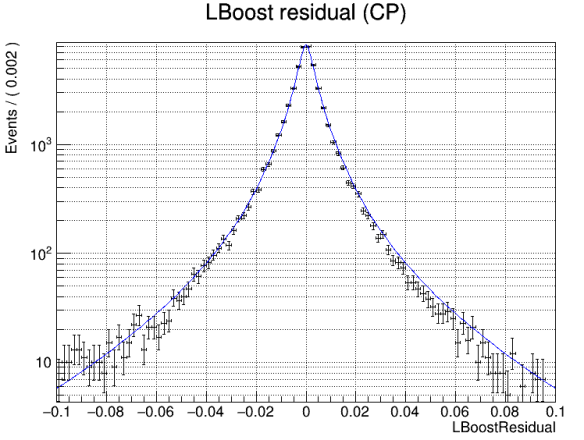
\includegraphics[height=5cm]{figures/residual0_10}	
	\end{subfigure}
	\begin{subfigure}{0.5\linewidth}
		\caption{$0<\chi^2/N<0.4$}
		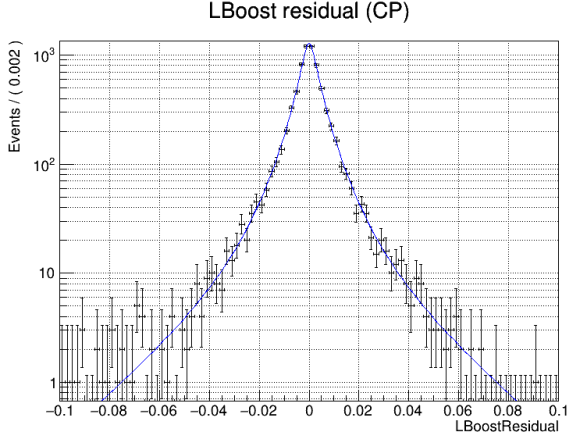
\includegraphics[height=5cm]{figures/residual0_0.4}
		%\caption{Tagging efficiency $\epsilon$ and $\mu$ in r-bins for $B^0 \to K_S^0  K_S^0  K_S^0$.}
	\end{subfigure}
	\begin{subfigure}{0.5\linewidth}
		\caption{$0.4<\chi^2/N<0.8$}
		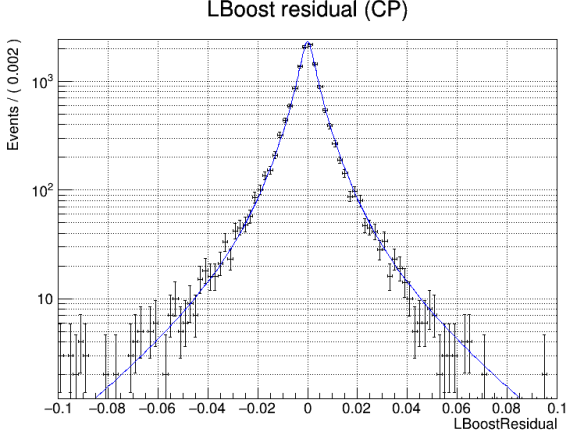
\includegraphics[height=5cm]{figures/residual0.4_0.8}
		%\caption{Tagging efficiency $\epsilon$ and $\mu$ in r-bins for $B^0 \to K_S^0  K_S^0  K_S^0$.}
	\end{subfigure}
	\begin{subfigure}{0.5\linewidth}
		\caption{$0.8<\chi^2/N<1.2$}
		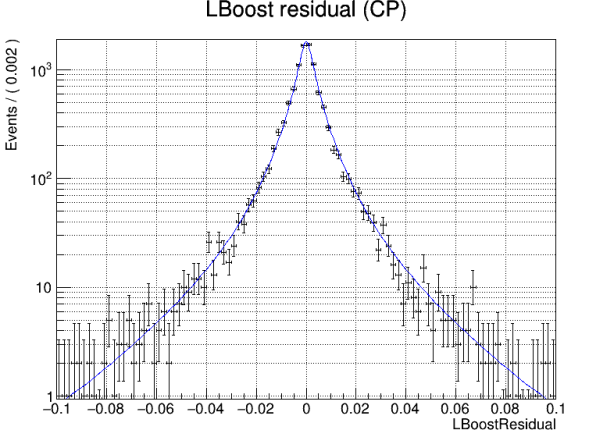
\includegraphics[height=5cm]{figures/residual0.8_1.2}
		%\caption{Tagging efficiency $\epsilon$ and $\mu$ in r-bins for $B^0 \to K_S^0  K_S^0  K_S^0$.}
	\end{subfigure}
	
	\begin{subfigure}{0.5\linewidth}
		\caption{$1.2<\chi^2/N<1.6$}
		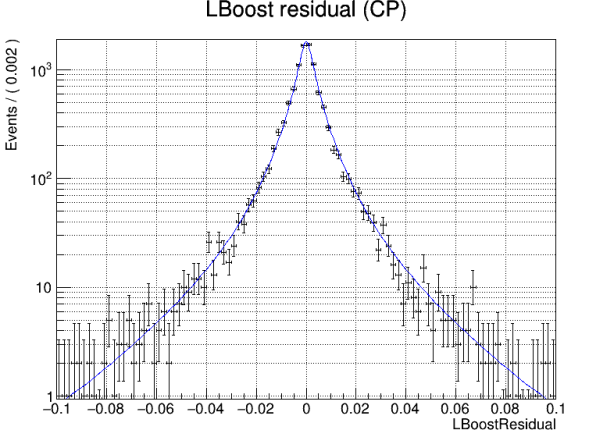
\includegraphics[height=5cm]{figures/residual1.2_1.6}
		%\caption{Tagging efficiency $\epsilon$ and $\mu$ in r-bins for $B^0 \to K_S^0  K_S^0  K_S^0$.}
	\end{subfigure}
	\begin{subfigure}{0.5\linewidth}
		\caption{$1.6<\chi^2/N<10$}
		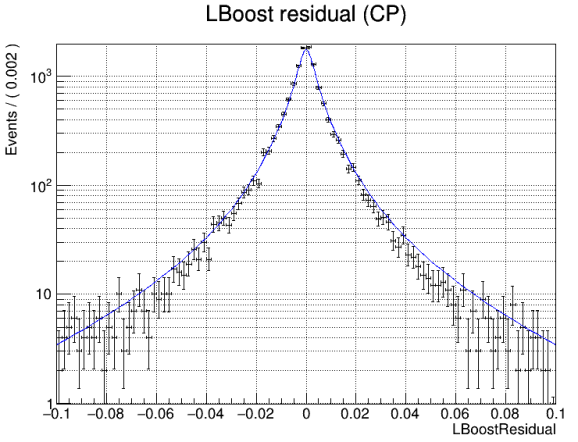
\includegraphics[height=5cm]{figures/residual1.6_10}
		%\caption{Tagging efficiency $\epsilon$ and $\mu$ in r-bins for $B^0 \to K_S^0  K_S^0  K_S^0$.}
	\end{subfigure}
	\caption{ The $z$ position residual of $B^0$ vertices on $\it{CP}$-side, which is dependent on the $\chi^2/N$. The first plot is the fit in the full range and the rest of the plots are the fit in each sliced range of $\chi^2/N$. The events are the true candidates taken from the \textit{signal MC}.}
	\label{fig:redchi2fit}
\end{figure}
\begin{comment}
\begin{table}[H]
\begin{minipage}[b]{1.0\linewidth}
\centering
\caption{Parameters in $R_{cp}$.}
\label{tab:Rcp}
\begin{tabular}{|c|c|}
\hline
$f_{cp}^{tail}$ & $0.0742 \pm 0.0008$\\
$s_0^{main}$&  $0.9151 \pm 0.0077$ \\
$s_1^{main}$ & $0.2142\pm 0.0064$\\
$s_0^{tail}$ &  $2.0477\pm 0.0779$\\
$s_1^{tail}$  & $1.3470\pm 0.0720$ \\
\hline
\end{tabular}
\end{minipage}
\end{table}
\end{comment}


\begin{table}[H]
	\begin{minipage}[b]{1.0\linewidth}
		\centering
		\caption{Parameters in $R_{cp}$.}
		\label{tab:Rcp}
		\begin{tabular}{|c|c|}
			\hline
			$f_{cp}^{tail}$ & $0.07420 \pm 0.00080$\\
			$s_0^{main}$&  $0.9151 \pm 0.0077$ \\
			$s_1^{main}$ & $0.2142\pm 0.0064$\\
			$s_0^{tail}$ &  $2.048\pm 0.078$\\
			$s_1^{tail}$  & $1.347\pm 0.072$ \\
			\hline
		\end{tabular}
	\end{minipage}
\end{table}

\subsection{Tag-side resolution function}

For the tag-side, the vertexing is done by using \textit{KFit} and no IP constraint used. Since the tag-side vertex reconstruction takes into account the tracks of the charged particles which may not be directly from the tag-side $B^0$ decay, the vertex position could be affected by both detector effects like the $\it{CP}$-side and the degradation of the secondary vertex. This effect is demonstrated in Figure \ref{fig:tagvet} where the tag-side vertex fit will give an estimated position of the vertex around the range of orange meshed area while the actual position of the primary vertex of tag-side $B$ meson should be in the area of the blue circle.

\begin{figure}[htpb]
\centering
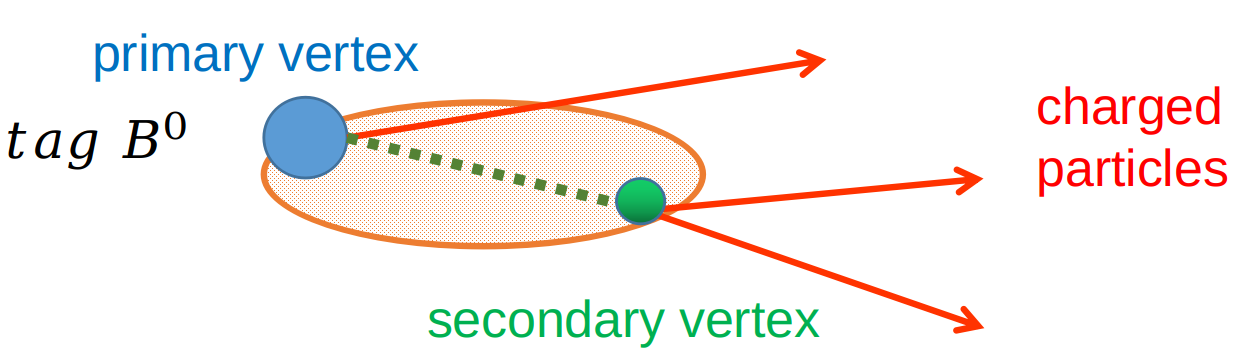
\includegraphics[width=0.9\linewidth]{tageffect}
\caption{The illustration of the tag-side $B^0$ vertex resolution affected by the non-primary tracks from the secondary vertex. The red arrows present the charged particles used for the tag-side vertex reconstruction, where one is from primary vertex of $B^0$ and two are from the secondary vertex.}
\label{fig:tagvet}
\end{figure}
To the contrary, if all tracks that are used for tag-side vertexing are primary tracks, the resolution will only be affected by the detector effects. The vertex position difference from the MC truth can be written as Equation \ref{eq:ztag}, where $\delta z_{tag}^{det}$ and $\delta z_{tag}^{np}$ are the position shifts caused by the detector effects and the vertex fit using non-primary tracks, respectively. Therefore, the effects from both detectors and non-primary tracks contributes to the total resolution on tag-side as shown in Equation \ref{eq:Rtag}.
\begin{equation}\label{eq:ztag}
\begin{split}
z_{tag} - z_{tag}^{'} =& (z_{tag}^{'} + \delta z_{tag}^{det} + \delta z_{tag}^{np}) - z_{tag}^{'}\\
=&\delta z_{tag}^{det} + \delta z_{tag}^{np}
\end{split}
\end{equation}
\begin{equation}\label{eq:Rtag}
R_{tag}( z_{tag}- z_{tag}^{'}) = R_{det}^{tag}(\delta z_{tag}^{det}) \otimes
R_{np}^{tag}( \delta z_{tag}^{np})
\end{equation}

Similarly to the $\it{CP}$-side resolution function, detector effects are presented as
\begin{equation}\label{eq:Rtagdet}
R_{det}^{tag}(\delta z_{tag}^{det}) = (1-f_{tag}^{tail})G(0,s_{tag}^{main}\cdot\sigma_{z_{tag}})+
f_{tag}^{tail}G(0,s_{tag}^{tail}\cdot\sigma_{z_{tag}})~,
\end{equation} where the main and tail Gaussian functions have the same mean value at zero, but the standard deviation is scaled by $\chi^2_{tag}/N$ on the tag-side:
\begin{equation}\label{eq:stag}
s_{tag}^{main/tail} = s_0^{main/tail} + s_1^{main/tail}\cdot\chi^2_{tag}/N~.
\end{equation} 
$R^{tag}_{det}$ can be obtained with MC samples of which tag-side tracks are all from a primary vertex. 

The fit model of $R_{np}^{tag}$ is shown in Equation \ref{eq:Rnp} which consists of three functions, including one Dirac $\delta$ function and two single-side exponential functions $E_p$ and $E_n$. The $E_p(x, y_p)=(1/y_p)e^{-x/y_p} $ when $x > 0$ and the $E_n(x, y_n)=(1/y_n)e^{x/y_n} $ when $x < 0$.
The exponential factors in both positive and negative components are scaled by the tag-side vertex uncertainty $\sigma_{z_{tag}}$. 
\begin{equation}\label{eq:Rnp}
R_{np}^{tag}(\delta z_{tag}^{np})=f_{\delta}\delta(\delta z_{tag}^{np}) + 
(1-f_{\delta})[f_p E_p(\delta z_{tag}^{np},\tau_p\cdot \sigma_{z_{tag}}) +
(1-f_p)E_n(\delta z_{tag}^{np},\tau_n\cdot \sigma_{z_{tag}}) ]
\end{equation} 


Since tag-side has no dependence on how $\it{CP}$-side is reconstructed, the resolution functions on tag-side are almost mode-independent. Thus these parameters are obtained by fitting to the control sample reconstructed from the MC. The control sample consists of multiple exclusive $D^{(*)}$ hadronic decays, of which the details are summarized in Appendix B. The control samples are also used in the analysis of $B^0\to J/\psi K^0_S$ study and the values of the parameters are referenced from the $B^0\to J/\psi K^0_S$ study~\cite{jpsiks_ichep}, too. The fit plots for tag-side resolution functions are shown in Figure \ref{fig:Rtagdet} and \ref{fig:Rtagnp}. The parameters obtained from the fit are listed in Table \ref{tab:Rtagdet} and Table \ref{tab:Rtagnp}.


\begin{figure}[H]
	\begin{minipage}[b]{0.5\linewidth}
		\centering
		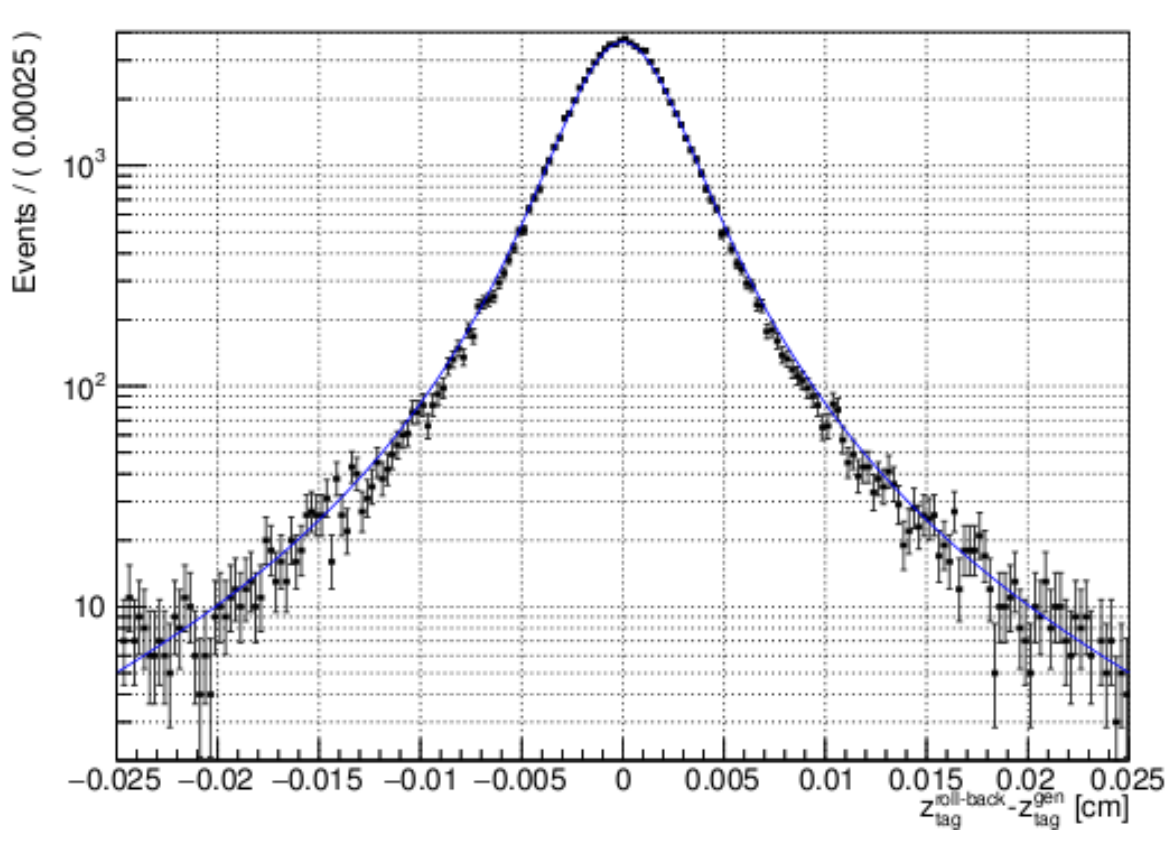
\includegraphics[height=5cm]{figures/Rdet}
		\caption{$R_{det}^{tag} $ fit}
		\label{fig:Rtagdet}
	\end{minipage}
	\begin{minipage}[b]{0.5\linewidth}
		\centering
		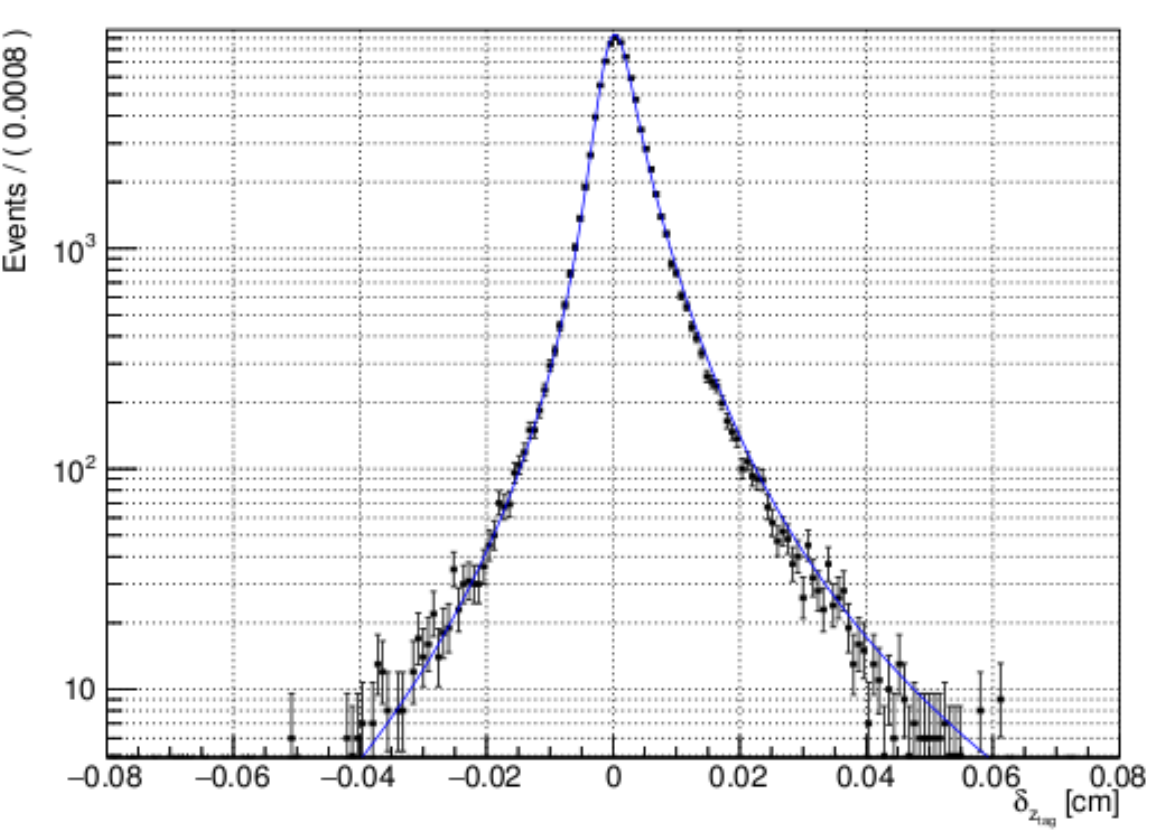
\includegraphics[height=5cm]{figures/Rnp}
		\caption{$R_{np}^{tag}$ fit}
		\label{fig:Rtagnp}
	\end{minipage}
\end{figure}
\begin{comment}
\begin{table}[H]
\begin{minipage}[b]{0.5\linewidth}
\centering
\caption{Parameters in $R^{tag}_{det}$}
\label{tab:Rtagdet}
\begin{tabular}{|c|c|}
\hline
$f_{tag}^{tail}$ & $0.0523 \pm 0.0025$\\
$s_0^{main}$&  $1.1446 \pm 0.0061$ \\
$s_1^{main}$ & $0.0443\pm 0.0022$\\
$s_0^{tail}$ &  $3.4480\pm 0.0897$\\
$s_1^{tail}$  & $0.2666\pm0.0276$ \\
\hline
\end{tabular}
\end{minipage}
\begin{minipage}[b]{0.5\linewidth}
\centering
\caption{Parameters in $R^{tag}_{np}$}
\label{tab:Rtagnp}
\begin{tabular}{|c|c|}
\hline
$f_{\delta}$ & $0.6256\pm 0.0049$\\
$f_p$ &  $0.8316 \pm 0.0051$ \\
$\tau_n$ & $2.9141\pm 0.0758$\\
$\tau_p$ &  $2.4846\pm 0.0269$\\
\hline
\end{tabular}
\end{minipage}
\end{table}
\end{comment}

\begin{table}[H]
	\begin{minipage}[b]{0.5\linewidth}
		\centering
		\caption{Parameters in $R^{tag}_{det}$}
		\label{tab:Rtagdet}
		\begin{tabular}{|c|c|}
			\hline
			$f_{tag}^{tail}$ & $0.0523 \pm 0.0025$\\
			$s_0^{main}$&  $1.1446 \pm 0.0061$ \\
			$s_1^{main}$ & $0.0443\pm 0.0022$\\
			$s_0^{tail}$ &  $3.448\pm 0.090$\\
			$s_1^{tail}$  & $0.267\pm0.028$ \\
			\hline
		\end{tabular}
	\end{minipage}
	\begin{minipage}[b]{0.5\linewidth}
		\centering
		\caption{Parameters in $R^{tag}_{np}$}
		\label{tab:Rtagnp}
		\begin{tabular}{|c|c|}
			\hline
			$f_{\delta}$ & $0.63\pm 0.05$\\
			$f_p$ &  $0.83 \pm 0.01$ \\
			$\tau_n$ & $2.914\pm 0.076$\\
			$\tau_p$ &  $2.485\pm 0.027$\\
			\hline
		\end{tabular}
	\end{minipage}
\end{table}

The boost direction is not exactly same in each event, while we use $\Delta t_i = \Delta z / \beta\gamma c$ as an universal relation to calculate the decay time difference for all the events, assuming the boosted direction of the CMS frame to the laboratory frame is always precisely along the $z$-direction for each event. It will cause a small additional contribution to the resolution of $\Delta t_i$, called kinematic effects. This effect could be reduced mainly by two approaches. First, instead of using the vertex position difference along the $z$-axis, we use the the relative distance between two vertices along the boosting direction calculated for each event during the vertex reconstruction. The second approach is to still use vertex position difference along the $z$-axis but introduce another resolution function called $R_k$ into Equation \ref{eq:tdcpv_all_res} for the kinematic correction of both signal and background events~\cite{tajima2004proper}. 
In the current stage of the Belle II, the dedicated study of $R_k$ is not ready because it requires a good understanding to the beam conditions and alignment in the event basis. Thus, the first approach is used in this thesis. 



\subsection{Background events $\Delta t$ distribution}
The $R_{bkg}$ model is approximately uncorrelated to vertex reconstruction method. Because the background component mainly comes from continuum events passing the selection, it is reasonable to model the vertex resolution of the background events by a Gaussian-like function. In this case, a double-Gaussian function with the standard deviations scaled by the measured uncertainties from both $\it{CP}$- and tag-sides is used as shown in Equation \ref{eq:Rbkg}. 
\begin{equation}\label{eq:Rbkg}
R_{bkg} = (1-f^{bkg}_{tail})G(\Delta t_i, \sigma^{bkg}_{main}\sqrt{\sigma^2_{z_{cp}}+\sigma^2_{z_{tag}}})
+ f^{bkg}_{tail}G(\Delta t_i, \sigma^{bkg}_{tail}\sqrt{\sigma^2_{z_{cp}}+\sigma^2_{z_{tag}}})
\end{equation}
where the $\sigma_{z_{cp}}$ and $\sigma_{z_{tag}}$ are the measured uncertainties of the vertex position in $\it{CP}$- and tag-sides. The $\sigma_{main}^{bkg}$ and $\sigma_{tail}^{bkg}$ are the non-unit scaling parameters which control the standard deviations of the main and tail Gaussian functions.

The shape of $\mathcal{P}_{bkg}\otimes R_{bkg}$ can be determined by fitting to the side-band data. The sideband region is defined as $M_{bc}<5.26$ GeV, according to Section 4.6. The requirement of $\Delta E$ is not used in the current definition of the sideband in order to increase the number of events, which will be added in future when more data is collected. Figure \ref{fig:Pbkg} shows the fit result using 60 sideband data. There are totally seven floating parameters to be determined which are all listed in Table \ref{tab:Pbkg}.
\begin{figure}[htpb]
	%	\begin{minipage}[b]{0.5\linewidth}
	%		\centering
	%		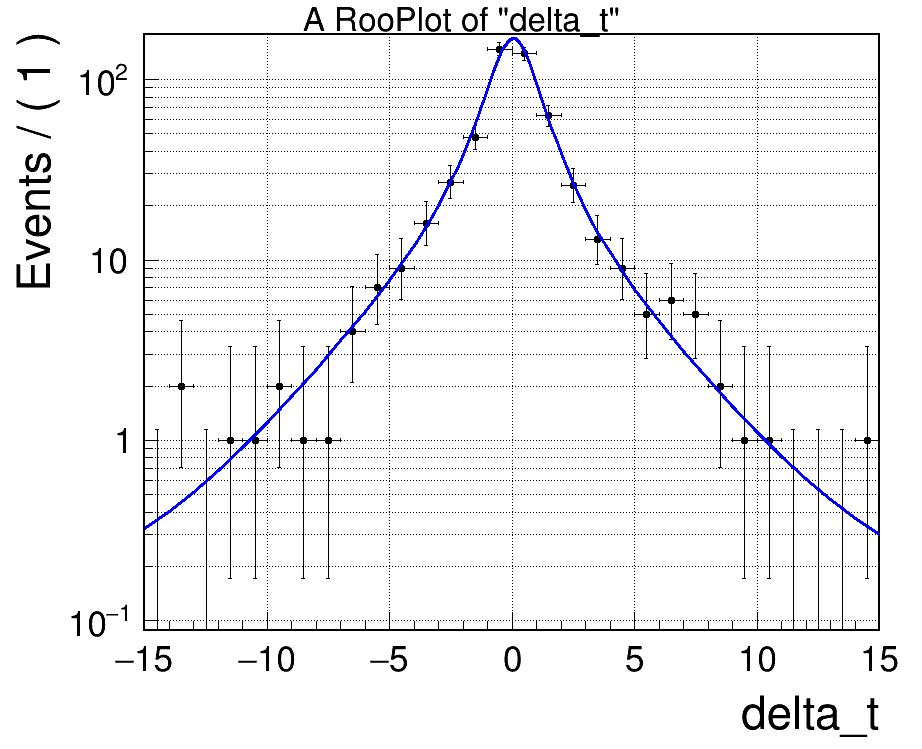
\includegraphics[height=5cm]{figures/bkg-cpfit-gen-mbc526}
	%		\caption{Background fit on generic sideband}
	%	\end{minipage}
	%	\begin{minipage}[b]{0.5\linewidth}
	\centering
	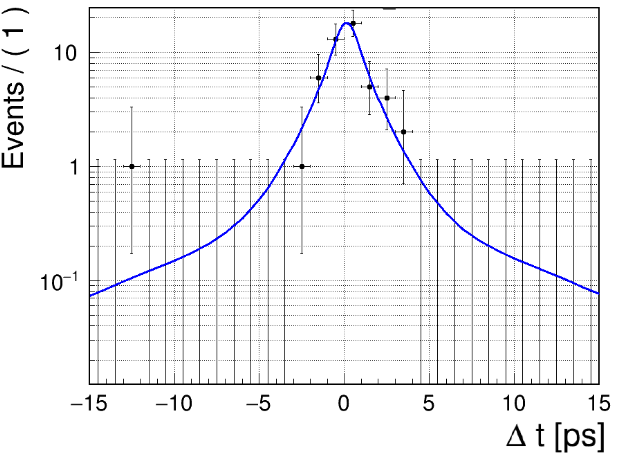
\includegraphics[height=5cm]{figures/bgres}
	\caption{$\mathcal{P}_{bkg}\otimes R_{bkg}$ fit  using 60 sideband events of the experiment data at $M_{bc} < 5.26$ GeV.}
	\label{fig:Pbkg}
	%	\end{minipage}
\end{figure}
\begin{comment}
\begin{table}[htpb]
\centering
\begin{tabular}{|c|c|}
\hline
$\mu^{bkg}_{\delta}$ & $0.1310 \pm 0.1902$\\
$\mu^{bkg}_{l}$&  $0.1638 \pm 0.5030$ \\
$\tau_{bkg}$ & $1.0541\pm 0.4370$\\
$f_{\delta}^{bkg}$ &  $0.5861\pm 0.2570$\\
$f^{bkg}_{tail}$  & $0.0417\pm 0.0408$ \\
$\sigma^{bkg}_{main}$ & $1.4348\pm 0.3940$\\
$\sigma^{bkg}_{tail}$ & $28.0930 \pm 8.8221$\\
\hline
\end{tabular}
\caption{Parameters in Background $\Delta t$ distribution. }
\label{tab:Pbkg}
\end{table}
\end{comment}


\begin{table}[htpb]
	\centering
	\begin{tabular}{|c|r|}
		\hline
		$\mu^{bkg}_{\delta}$ & $0.13 \pm 0.19$\\
		$\mu^{bkg}_{l}$&  $0.16 \pm 0.50$ \\
		$\tau_{bkg}$ & $1.05\pm 0.44$\\
		$f_{\delta}^{bkg}$ &  $0.59\pm 0.26$\\
		$f^{bkg}_{tail}$  & $0.04\pm 0.04$ \\
		$\sigma^{bkg}_{main}$ & $1.43\pm 0.39$\\
		$\sigma^{bkg}_{tail}$ & $28.1 \pm 8.8$\\
		\hline
	\end{tabular}
	\caption{Parameters in Background $\Delta t$ distribution. }
	\label{tab:Pbkg}
\end{table}

\section{Flavor Tagging}
 In order to determine the flavor of tag-side $B^0$, a flavor tagging algorithm has been developed. The flavor tagging uses information of charged particles including $\mu^{\pm}$, $\pi^{\pm}$,$K^{\pm}$ and $\Lambda^{}$. The same charged particles could be originated from the different mother particles in the tag-side decay, so that their importance to the determination of the flavor of the $B^0$ meson can be varied. For instance, a lepton from decay of $\bar{B^0}\to D^{*+}l^{-}\bar{\nu}_l$ is directly related to the flavor of the tag-side meson $B$, where the negative charge corresponds to a $\bar{B^0}$, that is, $q=-1$. While a lepton from a flavor-definite decay like $B^0\to J/\psi(\to l^+l^-) K^0_S$ on the tag-side is much less useful because the both flavor of $B$ could produce such a decay. Thus, these charged particles are first combined into a set of total 13 categories, as demonstrated in the Figure \ref{fig:flavortagger}. In this step, one particle is likely to be assigned into more than one categories, such as a $K^-$ from $D^0\to K^-\pi^+$, which belongs to both ``Kaon" and ``KaonPion" pair categories. A event-level classifier using FastBDT algorithm is implemented to identifier the likelihood of a particle in each category. Then, for each event, the responses of the event-level FastBDT classifier of the 13 categories are combined to form an combiner-level classifier to identify the flavor of the tag-side $B$ meson. For example, the decay $\bar{B^0}\to D^{*+}l^{-}\bar{\nu}_l$, as shown in the right side of the Figure \ref{fig:flavortagger}, can give high likelihood outputs in the event-level classifier in categories of ``Electron", ``KinLepton", ``Kaon", ``KaonPion", ``SlowPion", ``MaximumP" and ``Fast-Slow-Correlation". The rest of the categories will have relatively low outputs. With combiner-level classification, these 13 outputs could give an output of this decay being a  $\bar{B^0}$, so that the $\it{CP}$-side $B$ is much likely to be a $B^0$. 

\begin{figure}[H]
\centering
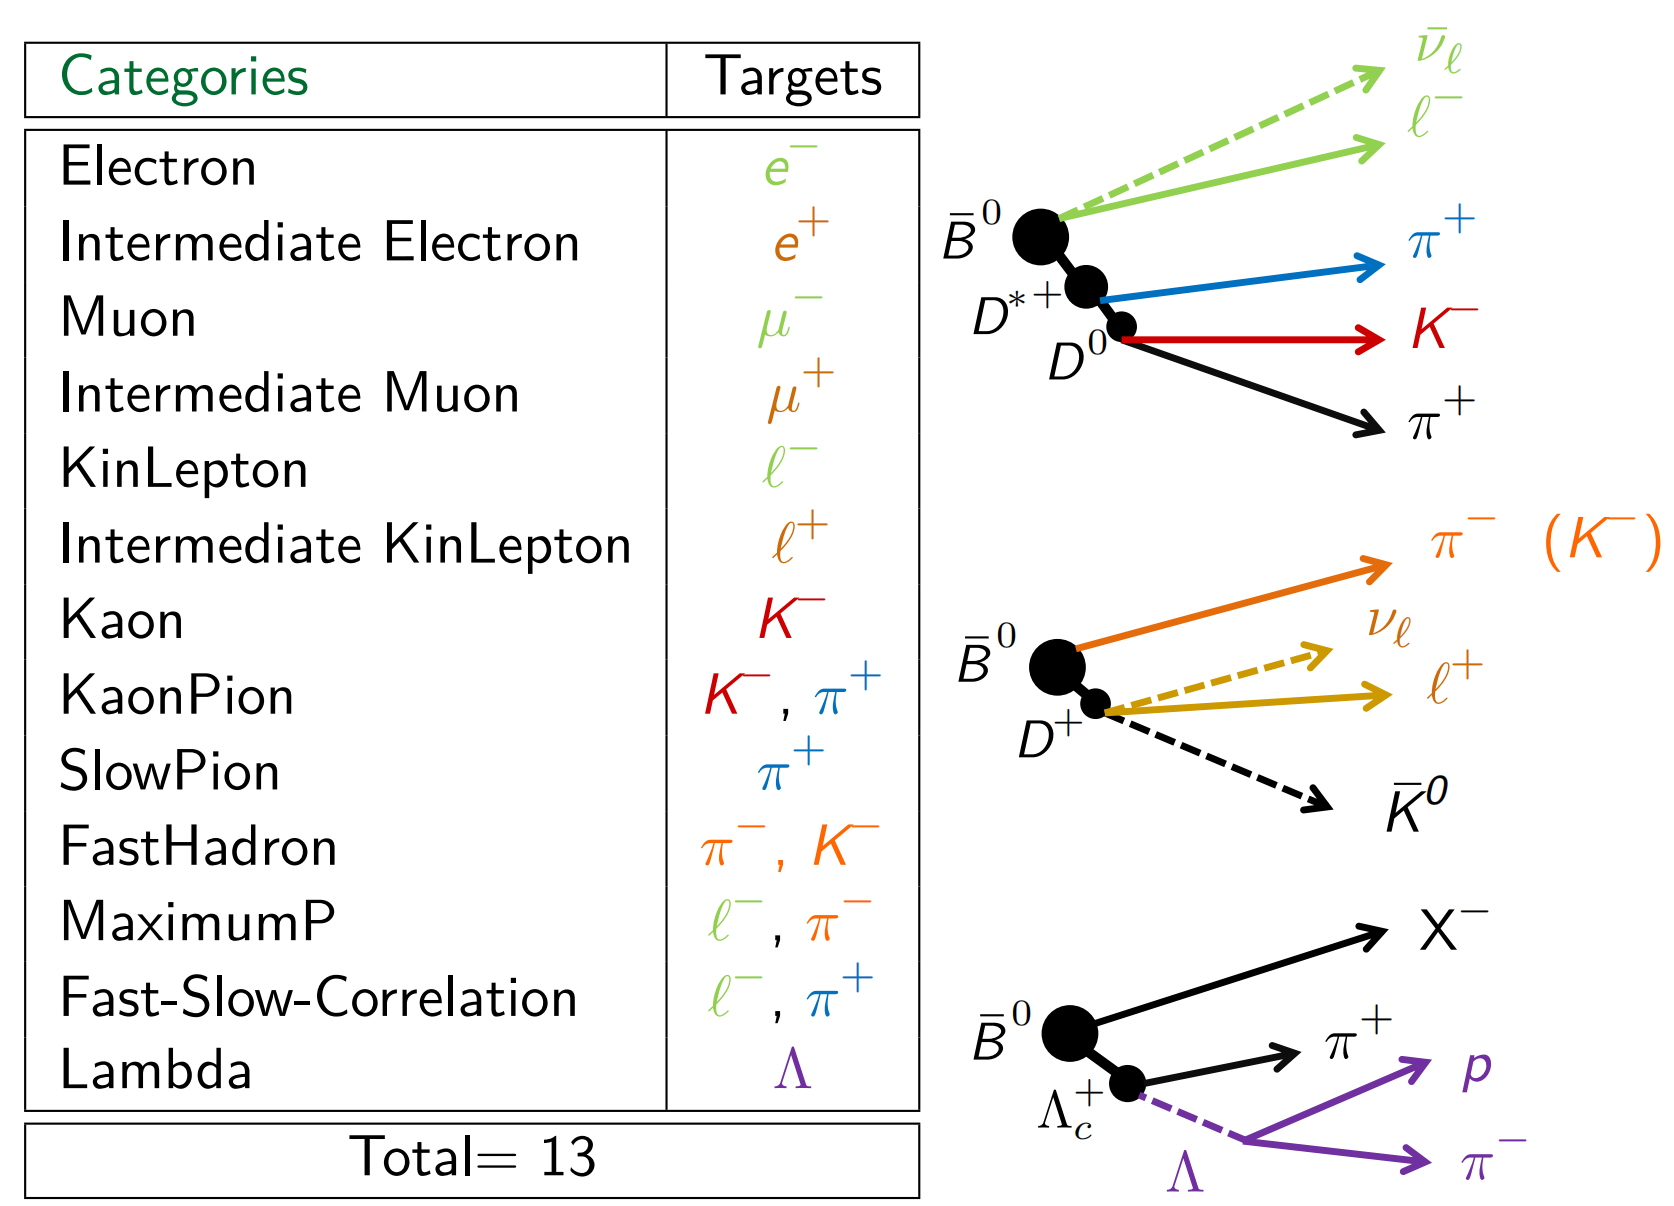
\includegraphics[width=0.7\linewidth]{tagger}
\caption{Particles and their categories used in flavor tagging algorithm~\cite{abudinen2020first}. The right side shows a few typical decay processes in the tag-side which are flavor definite and easy to be tagged. The color of the particles are corresponding to the possible categories they belong to in the particle-level classification.}
\label{fig:flavortagger}
\end{figure}
 
\begin{comment}
For each particle that has been used from above categories, PID and kinematics information are extracted and feed to the combiner as training variables, to obtained a classifier response corresponding to each category. Then for all responses from these categories, a total classifier is trained to present the likelihood of flavor $q$.
\end{comment}

This method is called category-based method and used in this thesis. To minimize impact of the reconstruction performance on $\it{CP}$-side, MC sample of $B^0 \to \nu \nu$ is used as the training sample where the final state in $\it{CP}$-side is completely invisible. 
Considering the limited power of flavor tagging accuracy, there is a certain fraction of events that are wrongly tagged. Thus, the flavor tagging efficiency $\epsilon$ and wrong tag fraction $w$ are introduced. Taking into account of the performance of the flavor tagging, the Equation \ref{eq:tdcpv_sig} turns into %Equation \ref{eq:tdcpv_all_ft}.

\begin{equation}\label{eq:tdcpv_all_ft}
\small
\mathcal{P}_{sig}^{obs}(\Delta t, q, \epsilon, w) = 
\frac{e^{-|\Delta t|/\tau_{B^0}}}{4\tau_{B^0}}
\epsilon
\begin{Bmatrix}
1 - q\cdot \Delta w+ q\cdot(1-2w)\cdot 
\begin{bmatrix}
\mathcal{S}\cdot\text{sin}(\Delta M_d \Delta t) + 
\mathcal{A}\cdot\text{cos}(\Delta M_d \Delta t)
\end{bmatrix}
\end{Bmatrix}~,
\end{equation} 
where $\epsilon$ is the flavor tagging efficiency, $w$ is the wrong tag fraction and $\Delta w = w_{B^0}-w_{\bar{B^0}}$ is the difference of the wrong tag fraction between $B^0$ and $\bar{B^0}$.
Compared to the original, the term with $\mathcal{S}$ and $\mathcal{A}$ is scaled by factor $r\equiv |1-2w|$, called  the dilution factor. The statistical uncertainty of $\mathcal{S}$ now becomes dependent to the tagging efficiency $\epsilon$ and wrong tag fraction $w$. 

The uncertainty of $w$ is much larger than $\epsilon$ so that $w$ gives an important source of systematic uncertainty. The validation of flavor tagger using flavor specific tagging control samples and Belle II data in 2019 is summarized in Ref.~\cite{abudinen2020first}. The $w$ for each single event is defined as a probability of being wrongly flavor tagged which can be presented by the average wrong tag fraction in a binned interval of the dilution factor. The binned values of dilution factor $r$ is defined for the calculation of $w$ as $[0.0, 0.1, 0.25, 0.5, 0.625, 0.75, 0.875, 1.0]$, also named as $r$-bin. For all events that have been successful tagged, they are projected into histogram of $r$-bin, and $w$ is calculated in each bin by the fraction of events of which the sign of the flavor tagger output is opposite to its true flavor. To easily use the information from the flavor tagger, the actual output of the flavor tagger is transformed into $q\cdot r$ where $q$ is the true flavor. In this case, an event with a small $w$ could give $r\simeq 1$ so that the flavor tagger output is close to its original flavor $q$, while $w>0.5$ can flip the sign of the $q$ indicating that this event is wrongly tagged with the opposite flavor. The distribution of $q\cdot r$ is shown in Figure \ref{fig:ft_qr} using \textit{signal MC}.

The distribution of $w$ and $\Delta w$ in each $r$-bin are shown in the top left and bottom left of the Figure \ref{fig:ft_wtag}, respectively. The $\Delta w$ is mostly within $3\%$, therefore the contribution from $\Delta w$ is treated as zero in Equation \ref{eq:tdcpv_all_ft} in this analysis. The distribution of $\epsilon$ and $\mu = \epsilon_{B^0}-\epsilon_{\bar{B^0}}$ in each $r$-bin are shown in the top right and bottom right of Figure \ref{fig:ft_wtag}, respectively. It is clear that the $\mu$ is mostly within a range of $\pm2\%$, also treated as zero in this thesis. We sum the $\epsilon$ for $B^0$ and $\bar{B^0}$ separately in all $r$-bins and take the average value to be used as the efficiency in Equation \ref{eq:tdcpv_all_ft} which is $(99.7\pm0.2)\%$, treated as 1 in this thesis. The performance of flavor tagger in $B^0 \to K_S^0  K_S^0  K_S^0$ and the ones from Ref.~\cite{abudinen2020first} are agreed, therefore the values of $w$ from tagging control samples is used in this thesis.

 \begin{figure}[htpb]
 	\centering
 	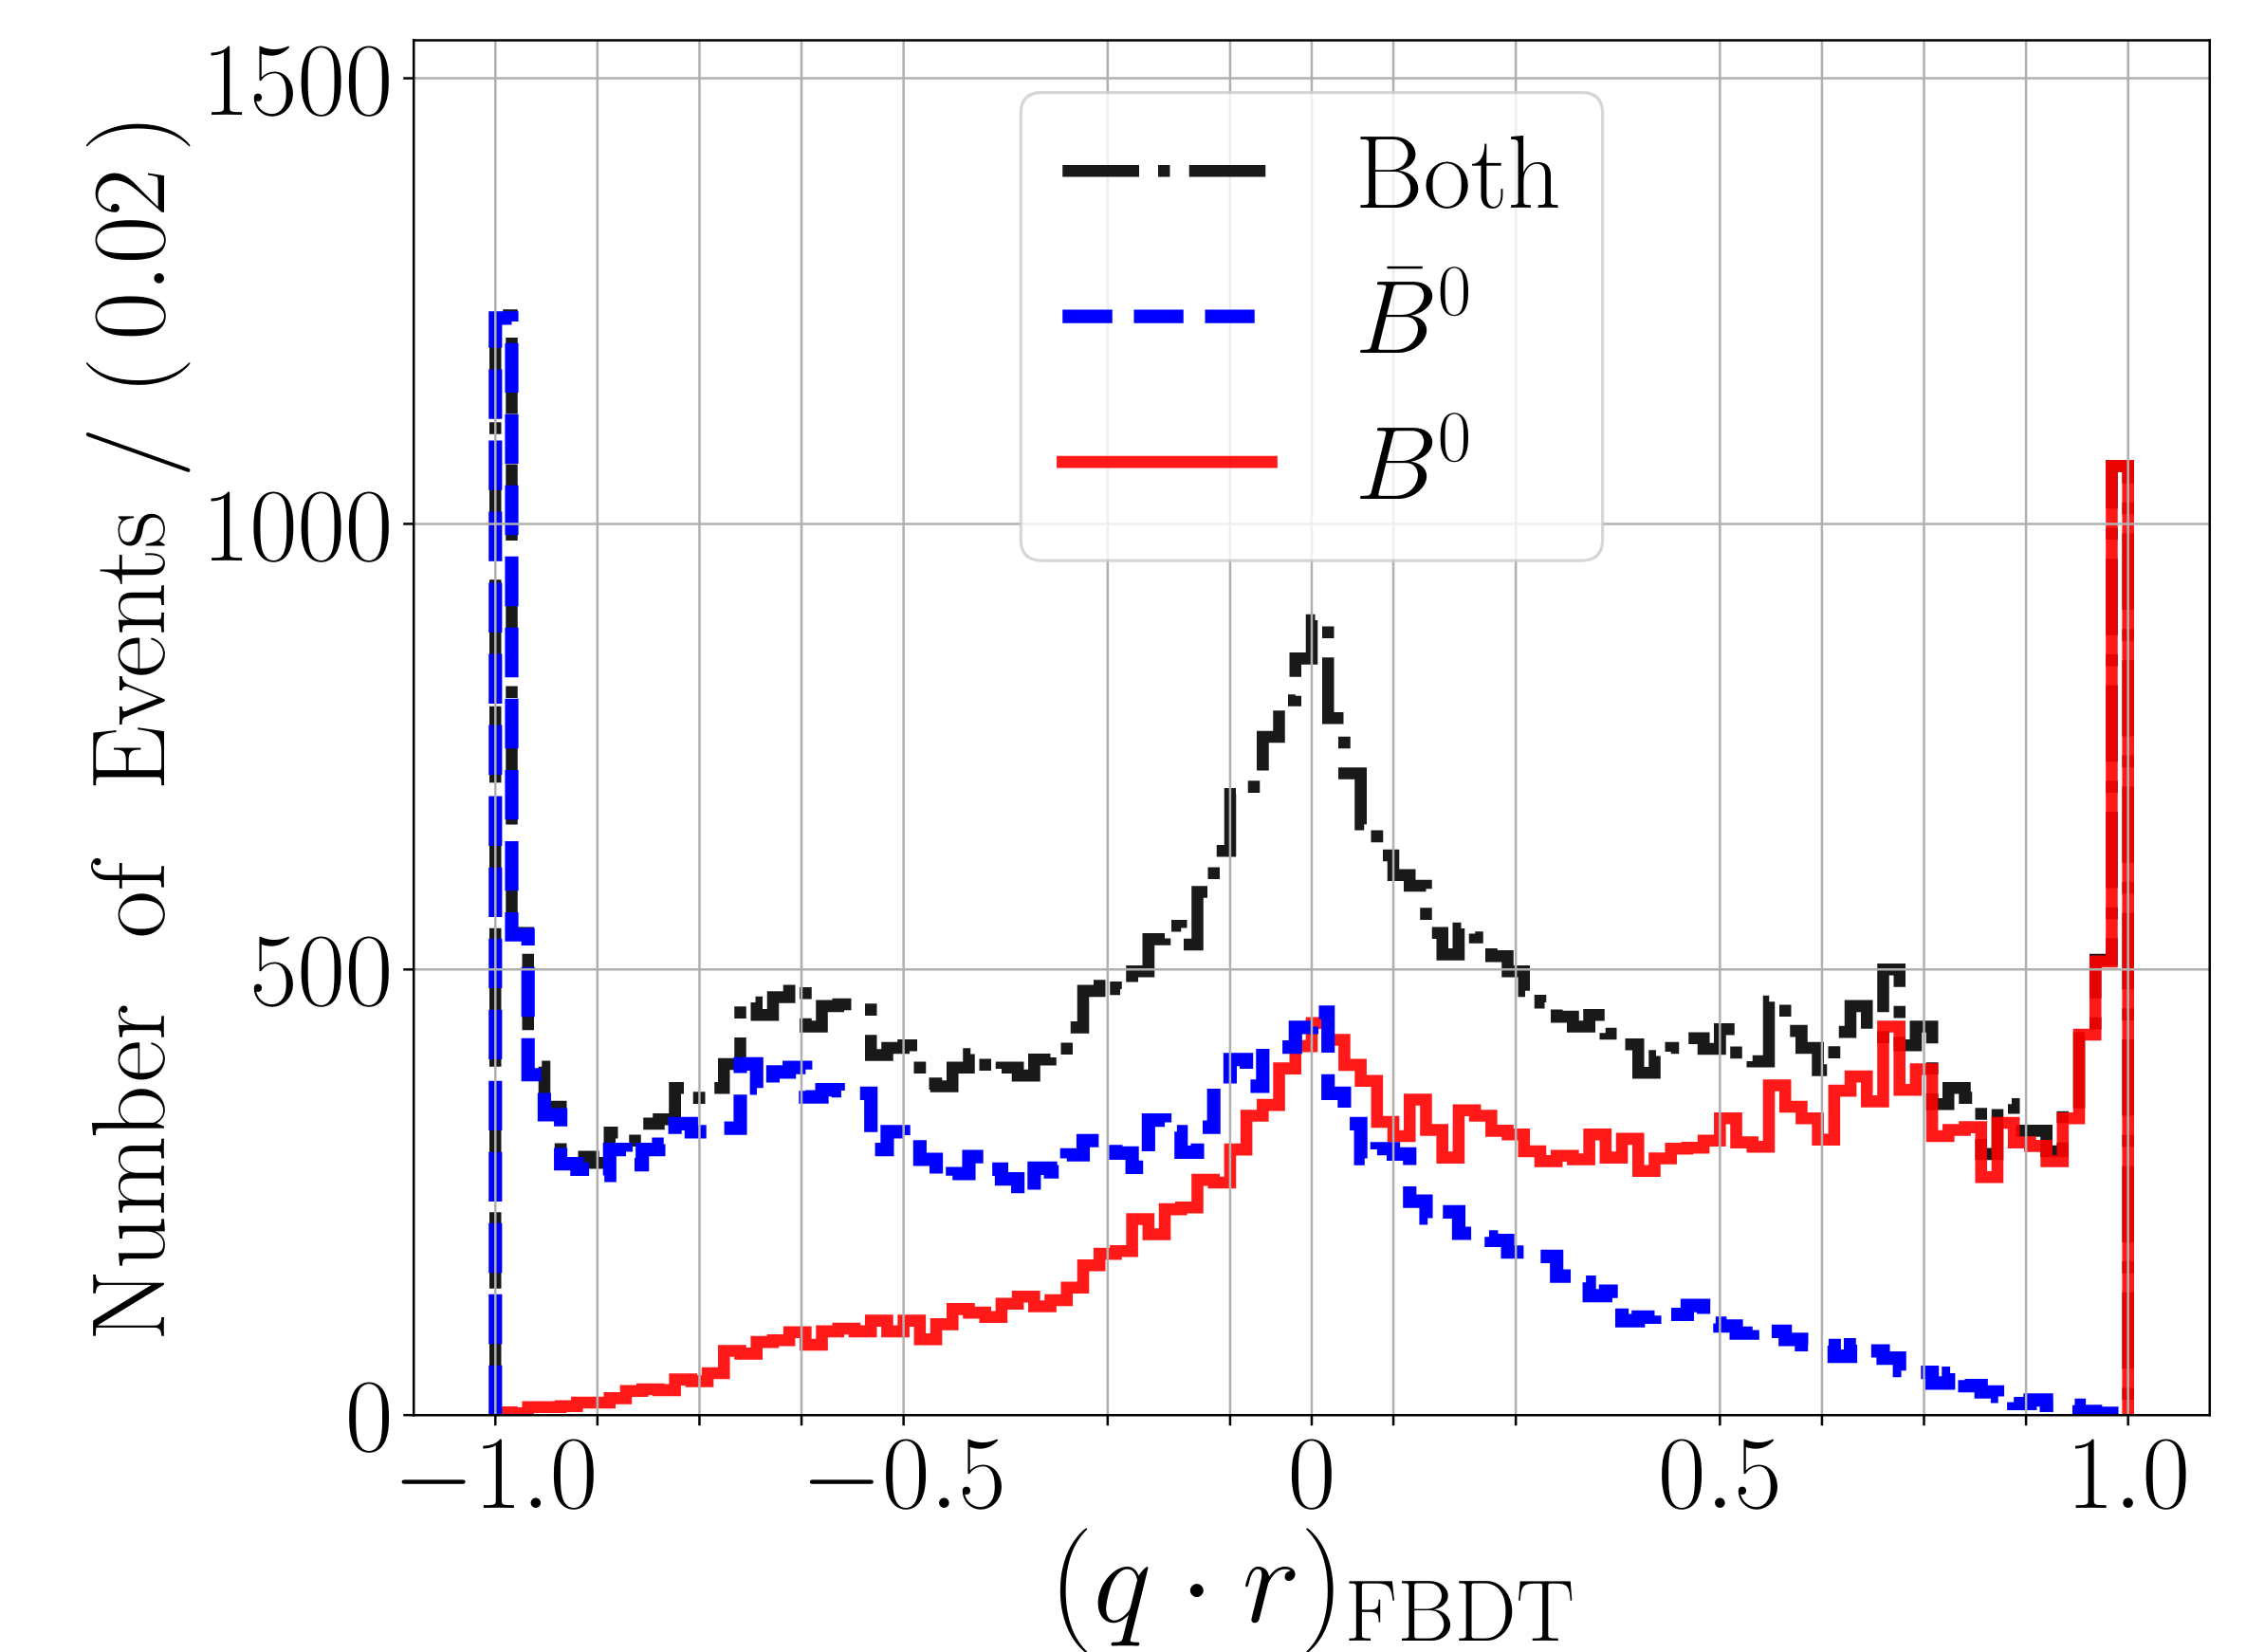
\includegraphics[width=0.7\linewidth]{figures/qr}
 	\caption{The distribution of flavor tagger output $(q\cdot r)$ for both tag-side of $B^0$ and $\bar{B^0}$ using \textit{signal MC}.}
 	\label{fig:ft_qr}
 	\end{figure}
 
 \begin{figure}[htpb]
 	\begin{subfigure}{0.5\linewidth}
 		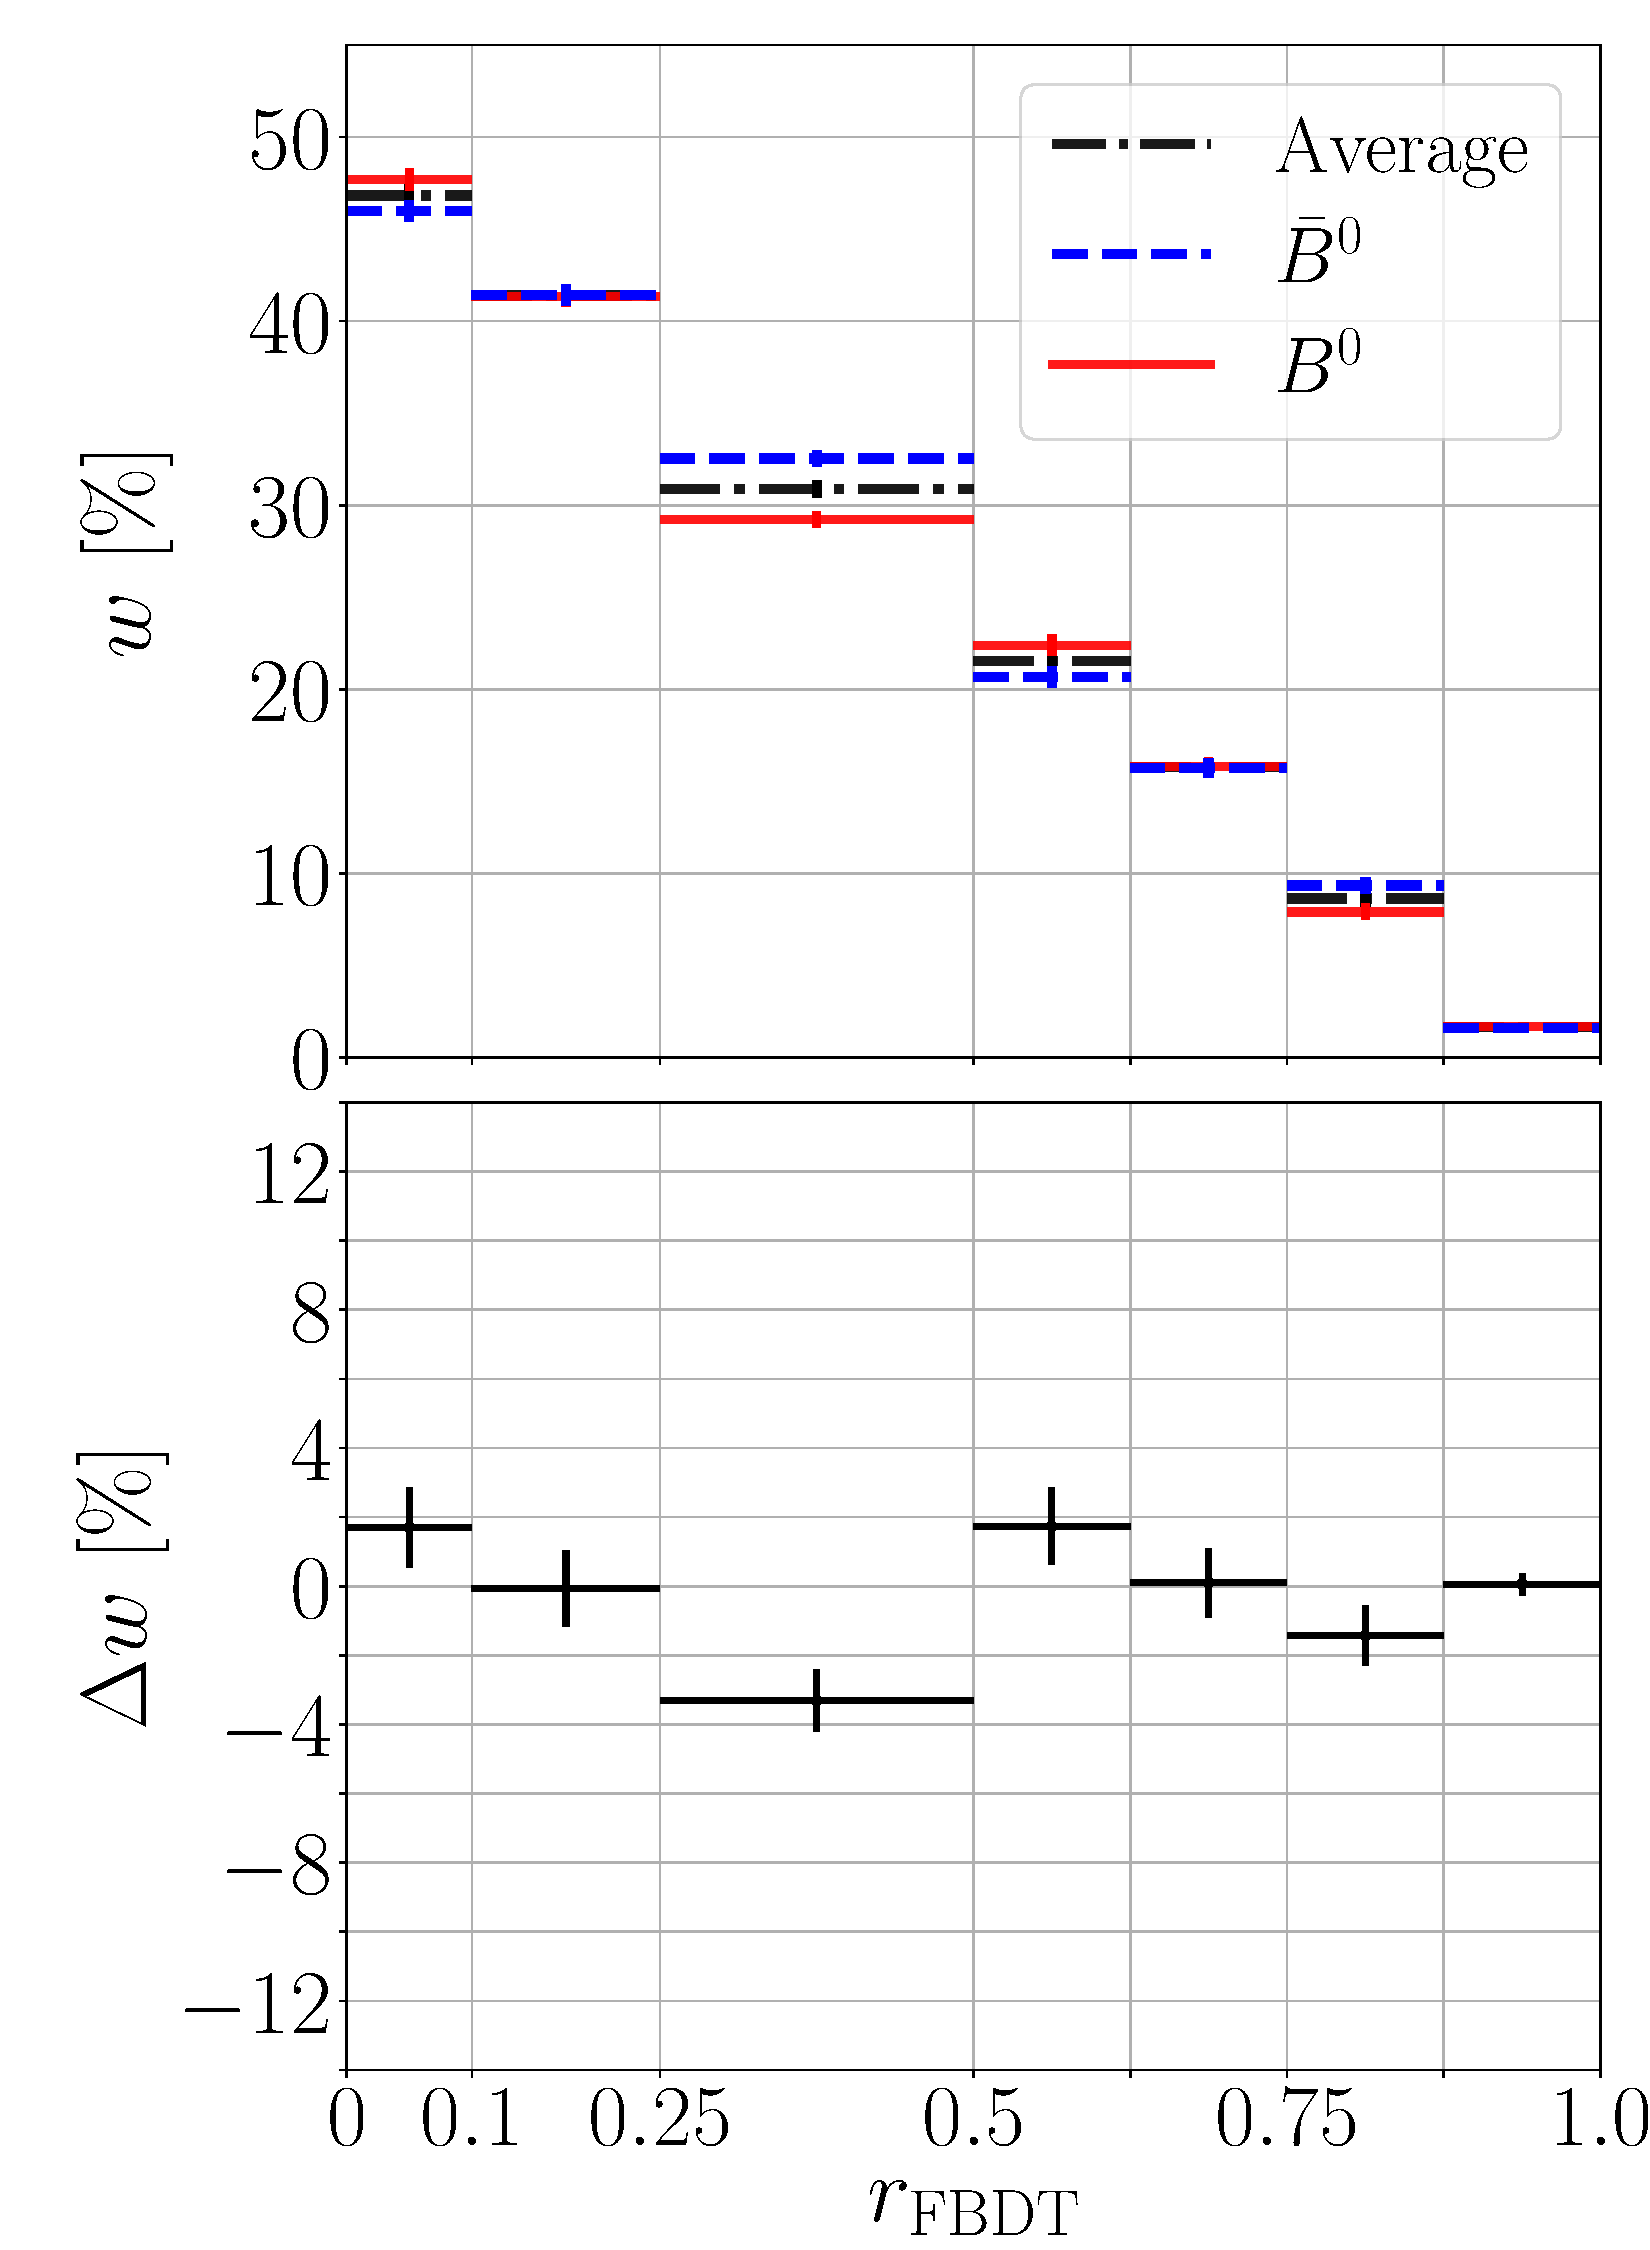
\includegraphics[width=1\linewidth]{pyFBDT_WrongTagFraction.pdf}
 	\end{subfigure}
 \begin{subfigure}{0.5\linewidth}
 	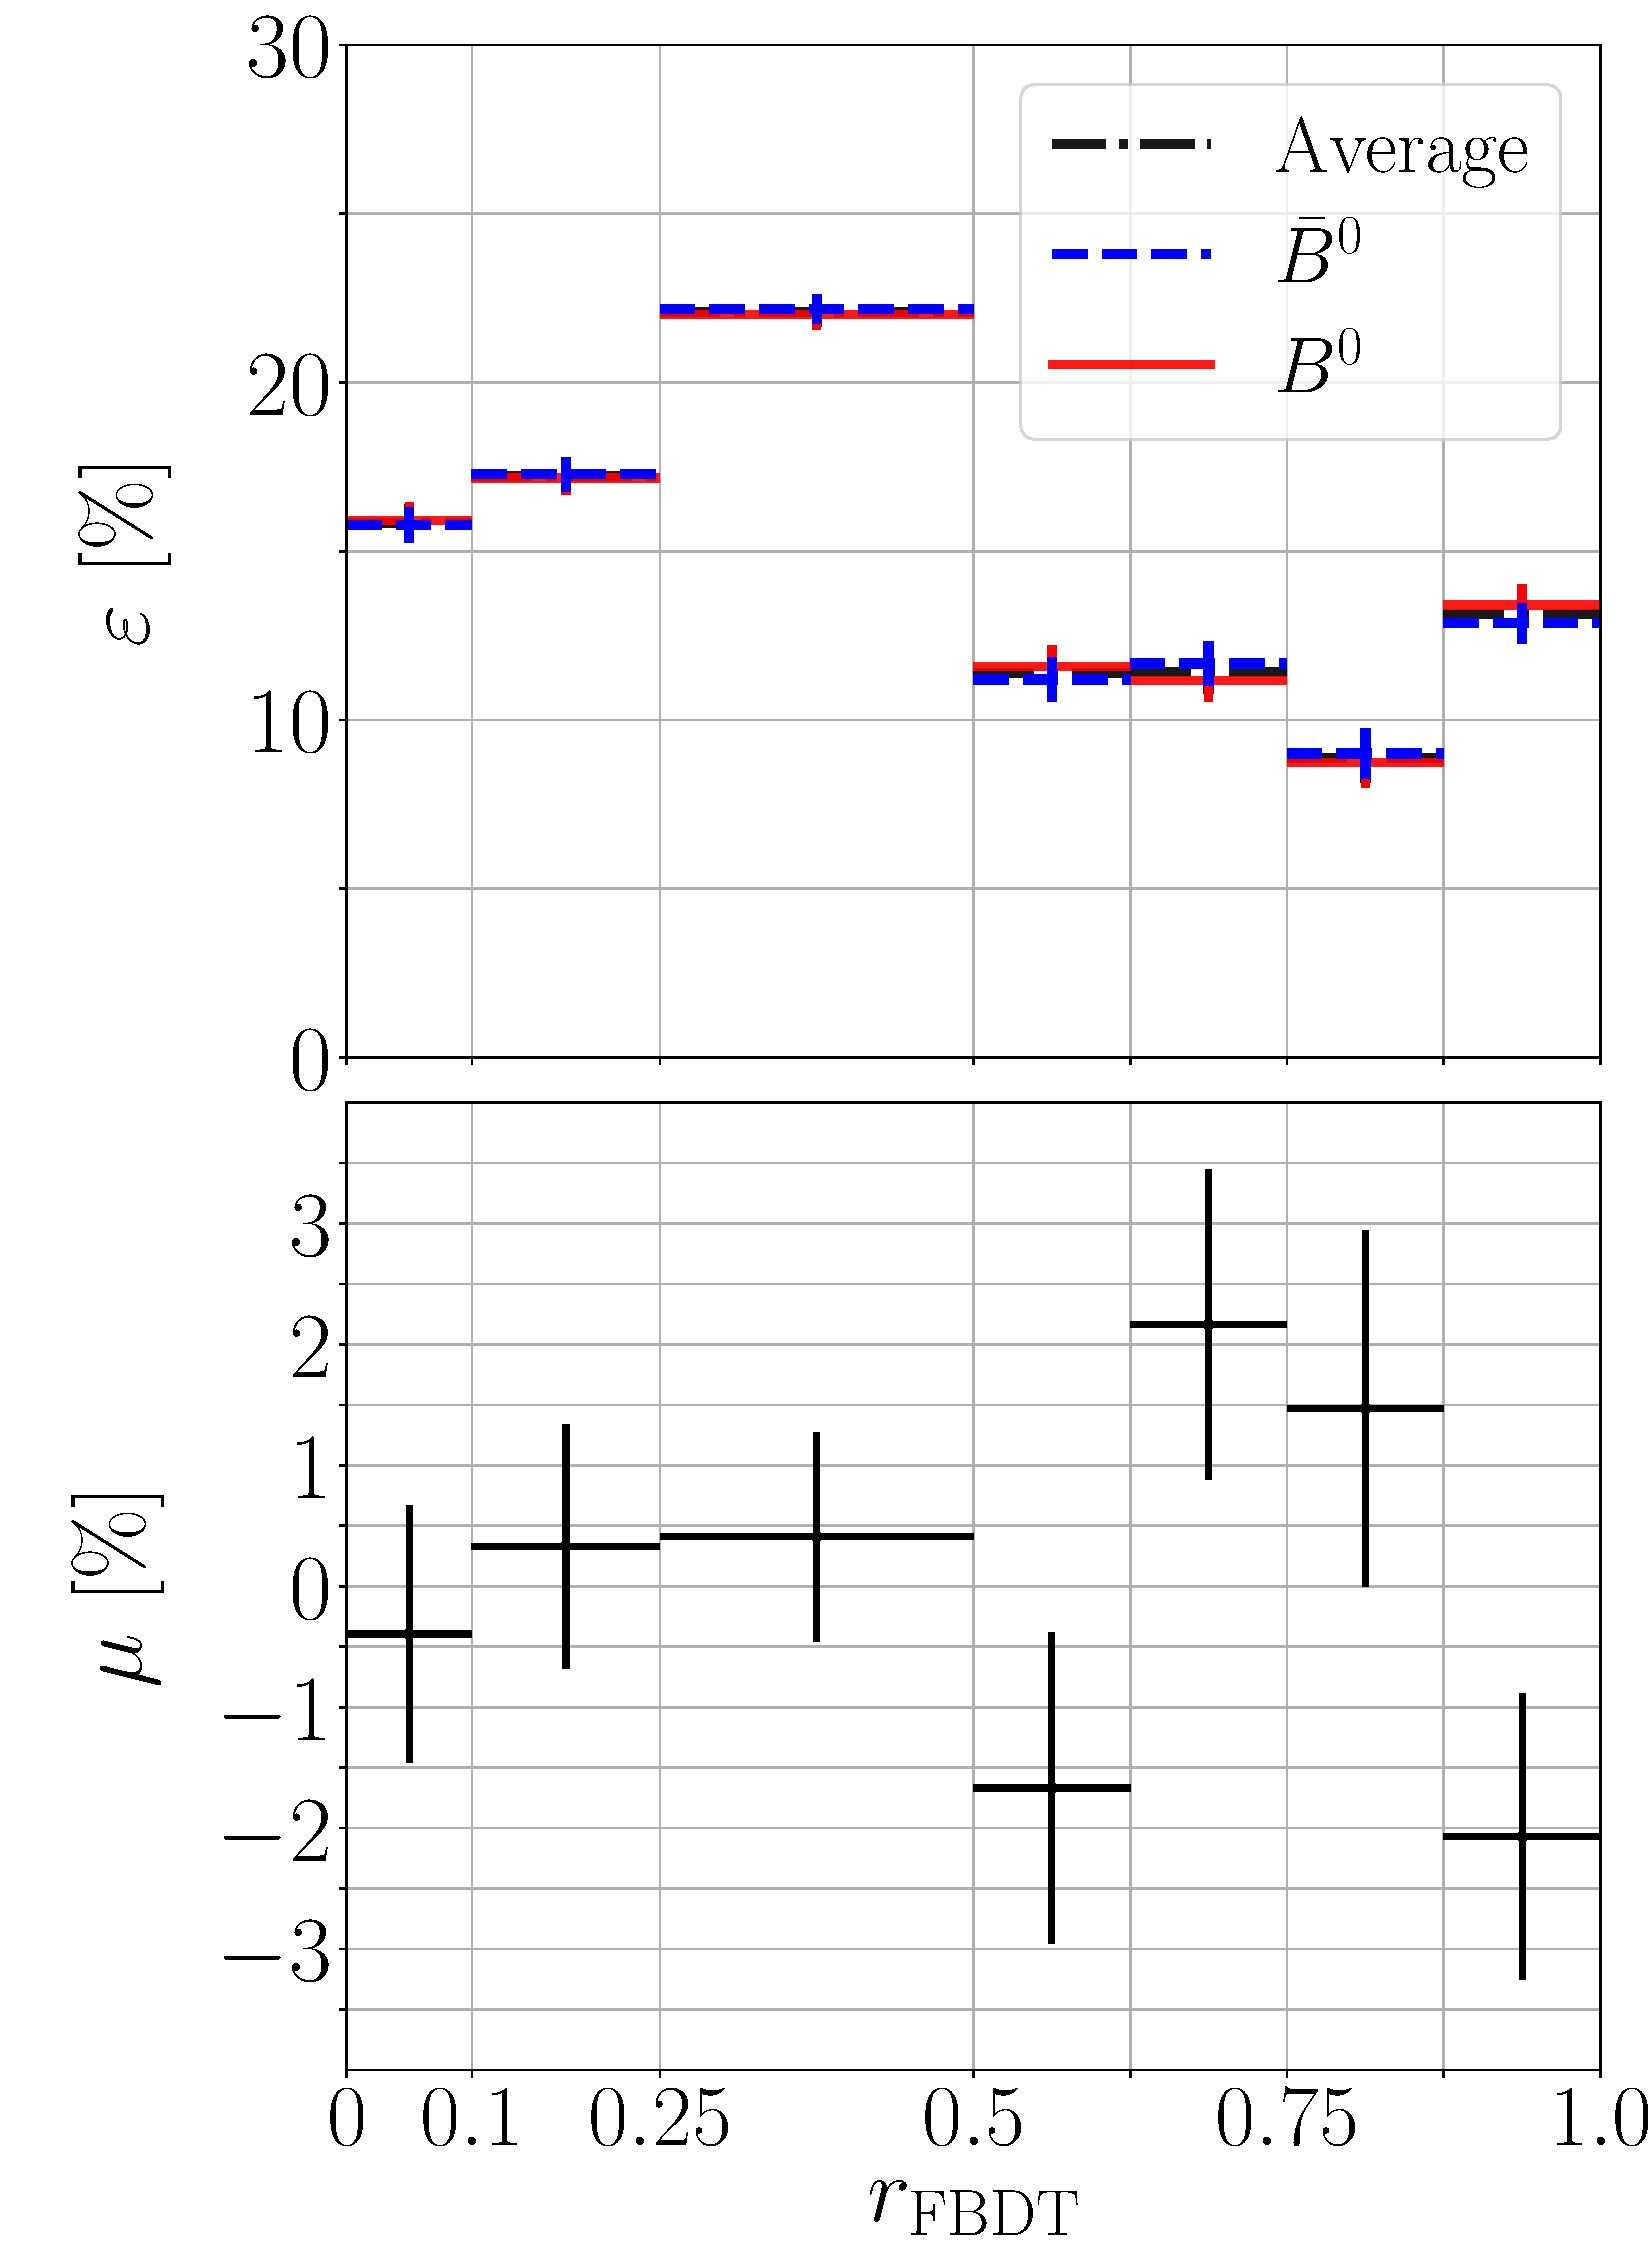
\includegraphics[width=1\linewidth]{pyFBDT_EfficiencyAndMu.pdf}
 \end{subfigure}
 	\caption{The flavor tagging efficiency, wrong tagging fraction, and their differences between different flavors sorted in each $r$-bin using \textit{signal MC}.}
 	\label{fig:ft_wtag}
 \end{figure}

\section{$\it{CP}$ Fitter}

The parameters that are needed for measuring $\mathcal{S}$ and $\mathcal{A}$ are studied and obtainable. Based on the observed $\Delta t$ distribution from selected events, Equation \ref{eq:tdcpv_all_res} can be fitted using the unbinned maximum likelihood method where $\Delta t$, signal fraction $f^{sig}$, and the flavor $q$ are taken as observables. The signal fraction for each event is calculated based on the $M_{bc}$ and $\Delta E$ values using the 2D fit model. In the meantime the vertexing error $\sigma_{z_{cp}}$, $\sigma_{z_{tag}}$ and $\chi^2/N$ are used as event-by-event conditional variables that are accessed during the fitting.
For Belle II, a new $\it{CP}$ fitter has been developed based on Python and RooFit, which is easy to use and integrated well with BASF2. The fitter requires a configuration file which contains all the parameter configurations including their ranges, initial values, floating states and uncertainties to perform the $\it{CP}$ parameter measurement. 

\begin{comment}
\begin{figure}[H]
\centering
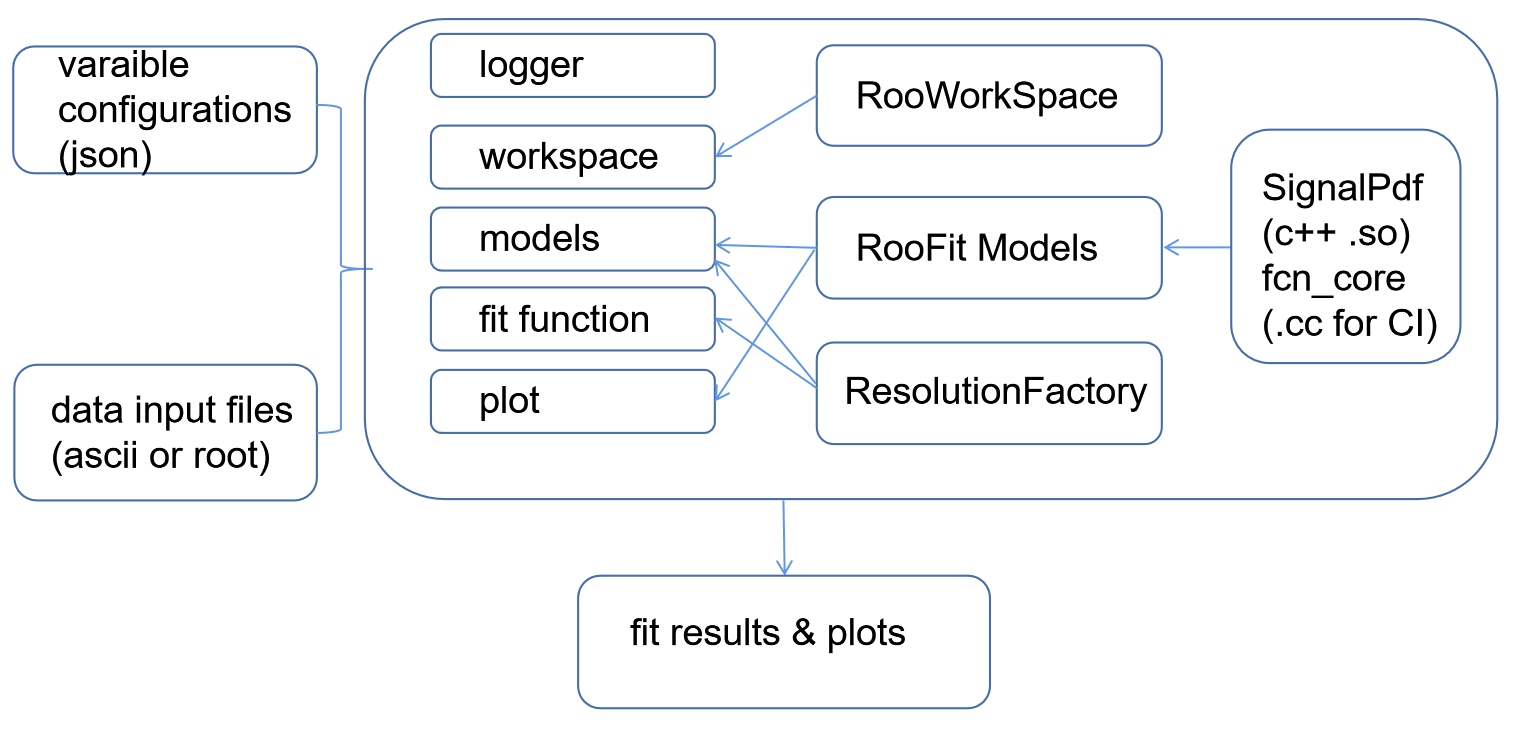
\includegraphics[height=6cm]{cpfitter-pict}
\caption{The structure of $\it{CP}$ fitter for Belle II. Users provide configuration file containing the definitions of all parameters and observables in the $\it{CP}$ fit. Data input files are used to create dataset for fitting. External library called ``SignalPdf.cxx" are generated in runtime to calculate the integral of resolutions and physics distribution event by event, which the fit is performed by maximizing the ``fcn\_core" function, presenting the likelihood of the dataset to the fit model. }
\end{figure}
\end{comment}



%2021/02/11 mid
\section{Blind analysis and fit}
As a required procedure to make sure the $\it{CP}$ parameters are measured without any bias due to the preconceived results, a blind analysis procedure is conducted before the fit is actually performed using the experimental data. The blind fit procedure includes the $\it{CP}$ fit on \textit{signal MC} and \textit{generic MC}, with different numbers of events used. To check the reliability of fit results from the $\it{CP}$ fitter, a linearity test and toy MC studies are also performed. 

\subsection{$\it{CP}$ fit on MC samples}
We first perform the $\it{CP}$ fit on events in \textit{signal MC} and \textit{generic MC}.
The \textit{signal MC} and \textit{generic MC} are generated with the phase-space model which contains zero $\it{CP}$ violation ($\mathcal{S}=\mathcal{A}=0$). In addition to the event selection criteria in the Table \ref{tab:b0select}, the cuts in Table \ref{tab:cutCP} are also applied for rejecting the events outside of the signal region and with very poor vertex reconstruction quality. Based on Section 4.6, the number of events inside the signal region is 30, which 26 events are kept after applying cuts in Table \ref{tab:cutCP}.
\begin{table}
	\centering
	\caption{The selection criteria for events that are used for $\it{CP}$ parameters fit.}
	\label{tab:cutCP}
\begin{tabular}{c|c}
	\hline
	Observables & Selections \\
	$\Delta t$ & $-70 < \Delta t < 70$ ps\\
	$\it{CP}$-side $\chi^2/N$ & $0 < (\chi^2/N)_{cp} < 8 $ \\
	tag-side $\chi^2/N$  & $0 < (\chi^2/N)_{tag} < 50 $\\
	$\sigma_{z_{tag}}$ &  $\sigma_{z_{tag}} < 0.1$ cm\\
	signal region & $5.27 < M_{bc} < 5.29$ GeV and $|\Delta E| < 0.1$ GeV\\
	\hline
\end{tabular}
\end{table}

We have 8873 events passing the selections from 10000 \textit{signal MC}. For 1 ab$^{-1}$ \textit{generic MC}, 373 events are selected to fit $\it{CP}$ parameters. To mimic the number of events expected in data sample, 26 events randomly sampled from \textit{generic MC} are used to perform the fit as well, which the sampling rounds take place for 100 times to avoid the large statistical fluctuations and the fit results are averaged. The $\it{CP}$ plots are shown in Figure \ref{fig:cpfitmc}. The fit results of $\mathcal{S}$ and $\mathcal{A}$ are summarized in Table \ref{tab:cpfit_result_mc}.

\begin{figure}[htpb]
	\begin{minipage}[t]{0.5\linewidth}
		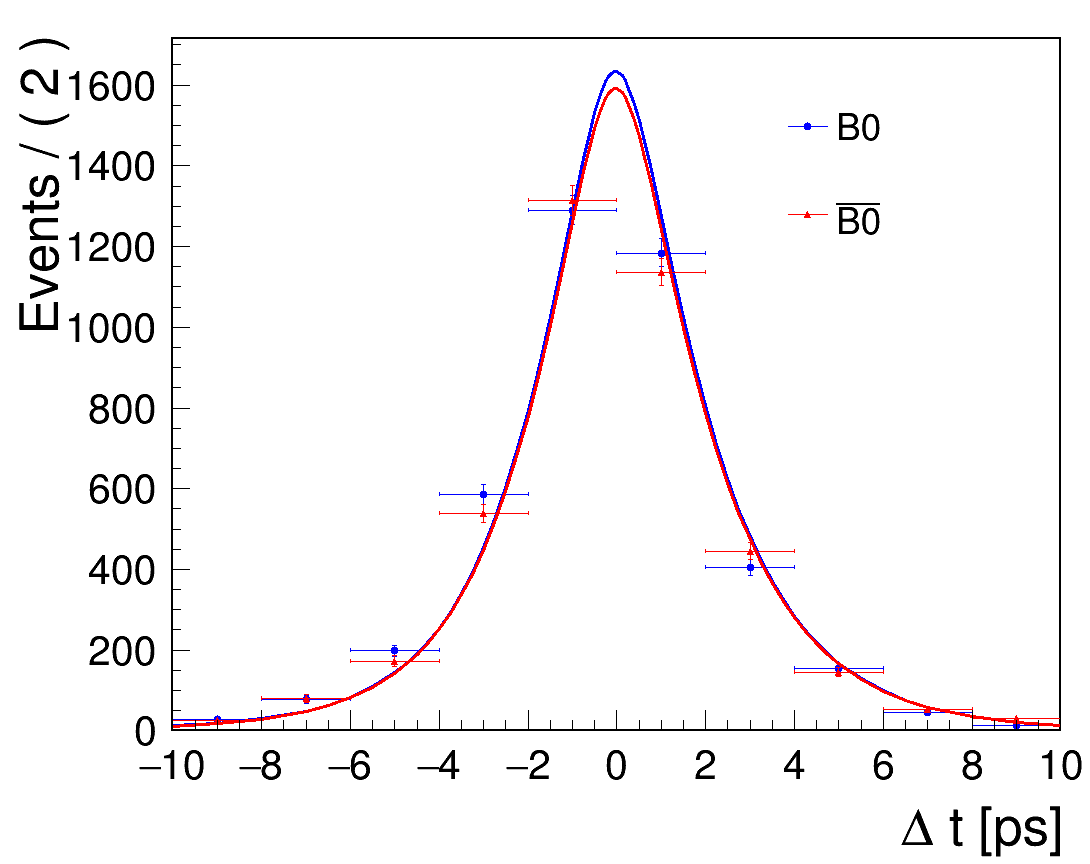
\includegraphics[height=5cm]{figures/cpfit-10000sig}
		%\caption{$\it{CP}$ fit on 8873 \textit{signal MC}.}
		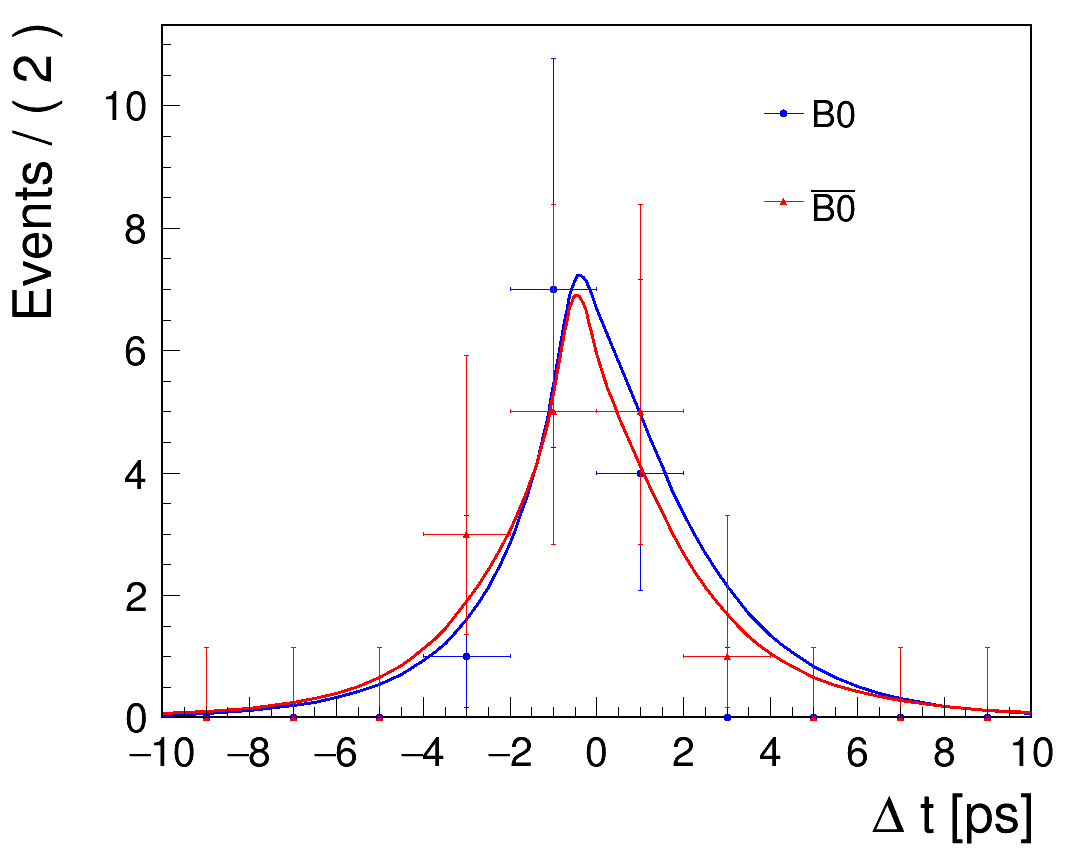
\includegraphics[height=5cm]{figures/cpfit-30gen}
		\label{fig:cpfit_sig}
	\end{minipage}
	\begin{minipage}[t]{0.5\linewidth}
		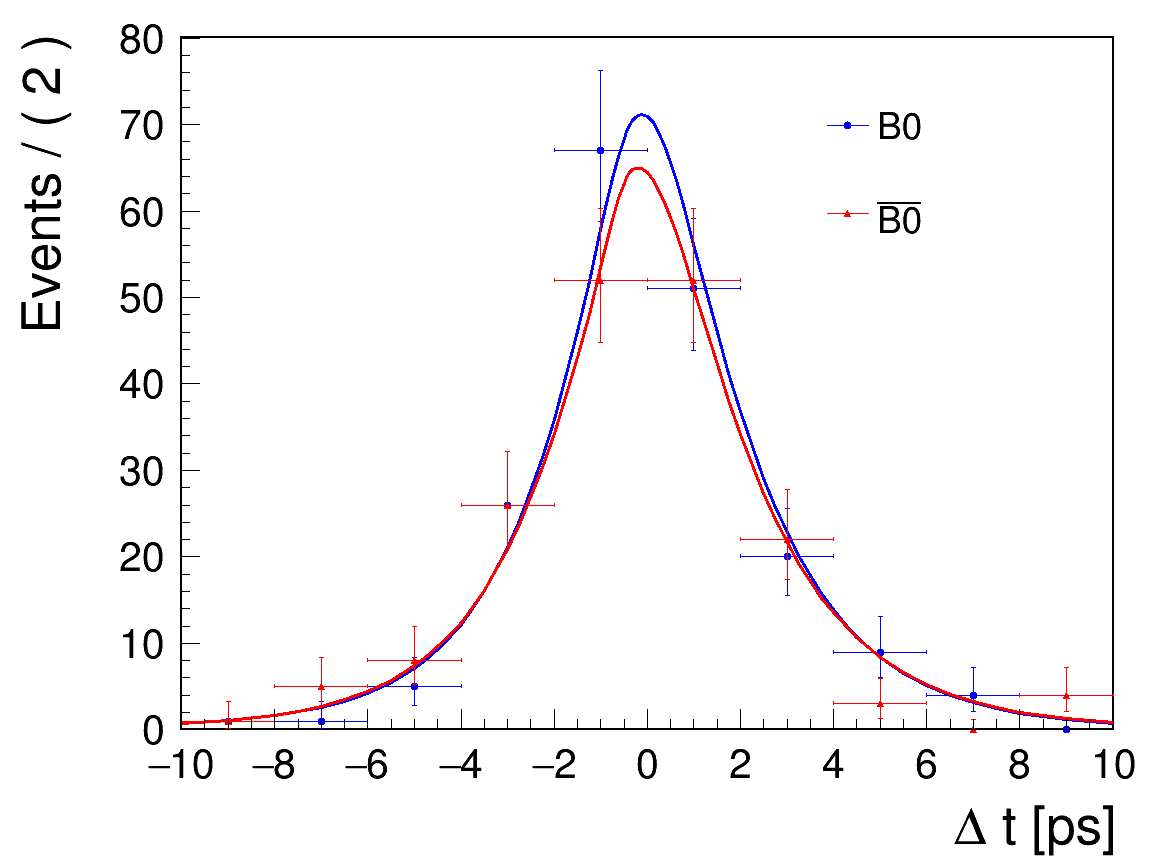
\includegraphics[height=5cm]{figures/cpfit-373gen}
		%\caption{$\it{CP}$ fit on 373 \textit{generic MC}.}
		\label{fig:cpfit_gen}
	\end{minipage}
\caption{The distribution of $\Delta t$ with the $\it{CP}$ fit. The top left is for \textit{signal MC} and the top right is for \textit{generic MC}. The bottom left is the fit of the first sampling round of 30 events of \textit{generic MC}.  }
\label{fig:cpfitmc}
\end{figure}


\begin{table}
	\centering
	\caption{The $\it{CP}$ fit results using \textit{signal MC} and \textit{generic MC} with only statistical uncertainties. The first two rows are the results from single time fit and the third is the average result from totally 100 times fit.}
	\label{tab:cpfit_result_mc}
\begin{tabular}{|c|c|c|}
	\hline
	Sample (events)& $\mathcal{S}$ &  $\mathcal{A}$\\
	\hline
	\textit{signal MC} (8873) & sin$(2\phi_1) = 0.00 \pm 0.04 $ &  $\mathcal{A} = -0.01 \pm 0.02$\\
	\hline
	\textit{generic MC} (373) &  sin$(2\phi_1)  = 0.00 \pm 0.21$ & $\mathcal{A}  = -0.05 \pm 0.07$ \\
	\hline
	\textit{generic MC} (30) & sin$(2\phi_1) = 0.20 \pm 0.85 $& $\mathcal{A} = -0.06 \pm 0.30$ \\
	\hline
\end{tabular}
\end{table}
\begin{comment}
The fit result for 8873 signal MC is:
\begin{equation}
\begin{split}
sin(2\phi_1) & = 0.00 \pm 0.04 \\
\mathcal{A} & = -0.01 \pm 0.02\\
\end{split}
\end{equation} 
the fit result for 373 generic MC is:
\begin{equation}
\begin{split}
sin(2\phi_1) & = 0.00 \pm 0.21 \\
\mathcal{A} & = -0.05 \pm 0.07\\
\end{split}
\end{equation} 
the fit result for 30 events generic MC is:
\begin{equation}
\begin{split}
sin(2\phi_1) & = 0.20 \pm 0.85 \\
\mathcal{A} & = -0.06 \pm 0.30\\
\end{split}
\end{equation} 
\end{comment}

The fit results are consistent with the expectation of non-$\it{CP}$ violation, and the statistical uncertainties are basically proportional to the $\sim 1/\sqrt{N}$, where $N$ is the number of events used for $\it{CP}$ fit. To test a fit on non-zero $\it{CP}$ violating MC, the fit on $B^0\to J/\psi K_S^0$ \textit{signal MC} is also done, of which the details of the event selection and the fit model determination can be found in Ref.~\cite{jpsiks_ichep}. The fit result over 10000 events is shown in Figure \ref{fig:cpfit_jpsiks}, which gives sin$(2\phi_1) = 0.70 \pm 0.05 $ and $\mathcal{A} = -0.01\pm 0.02$. The results agree with the inputs of $\mathcal{S}=sin(2\phi_1)=0.670$ and $\mathcal{A}=0$.
\begin{figure}[htpb]
	\centering
	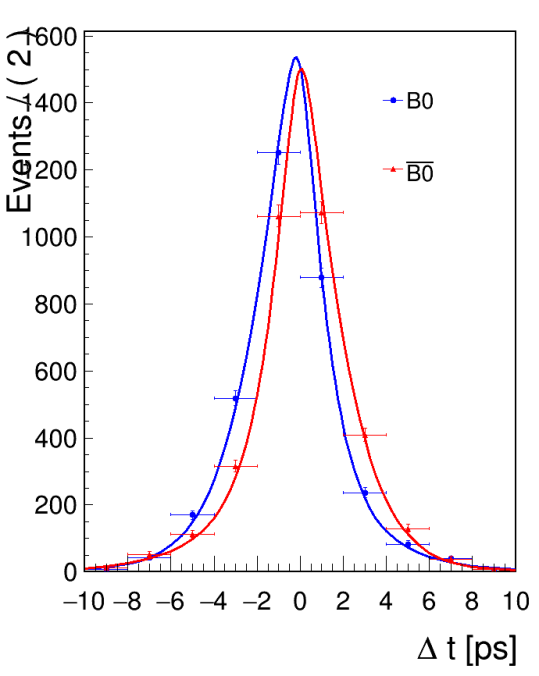
\includegraphics[width=6cm, height=6cm]{figures/jpsiks_cpfit10000}
	\caption{$\it{CP}$ fit over 10000 $B^0\to J/\psi K_S^0$ \textit{signal MC}.}
	\label{fig:cpfit_jpsiks}
\end{figure}
%We test the $\it{CP}$ fit on the sideband data with $M_{bc} < 5.27$ GeV.

\subsection{Linearity Test}
To validate the $\it{CP}$ fit linearity, a set of toy MC samples is generated where the $\chi^2$ from vertex fit and the vertex errors on $\it{CP}$- and tag-side are sampled from \textit{signal MC} as the conditional variables, while the number of events used in each toy MC sample is kept as 26 that is the same as data. The resolution function parameters are kept the same as $\it{CP}$ fit on \textit{generic MC}. The input $\mathcal{A}$ is set to zero while the input value of sin$(2\phi_1)$ is running from 0.1 to 0.9. For each value of input sin$(2\phi_1)$, 200 toy MC samples are generated. The center value and the error for sin$(2\phi_1)$ and $\mathcal{A}$ are determined by the mean and its uncertainty for each input from the fit using Gaussian function.
The dependence between input and output are shown in Figure \ref{fig:cpfit_line_S} where a linear function is used to fit the dependence with the uncertainties.
\begin{figure}[htpb]
	\begin{minipage}{0.5\linewidth}
		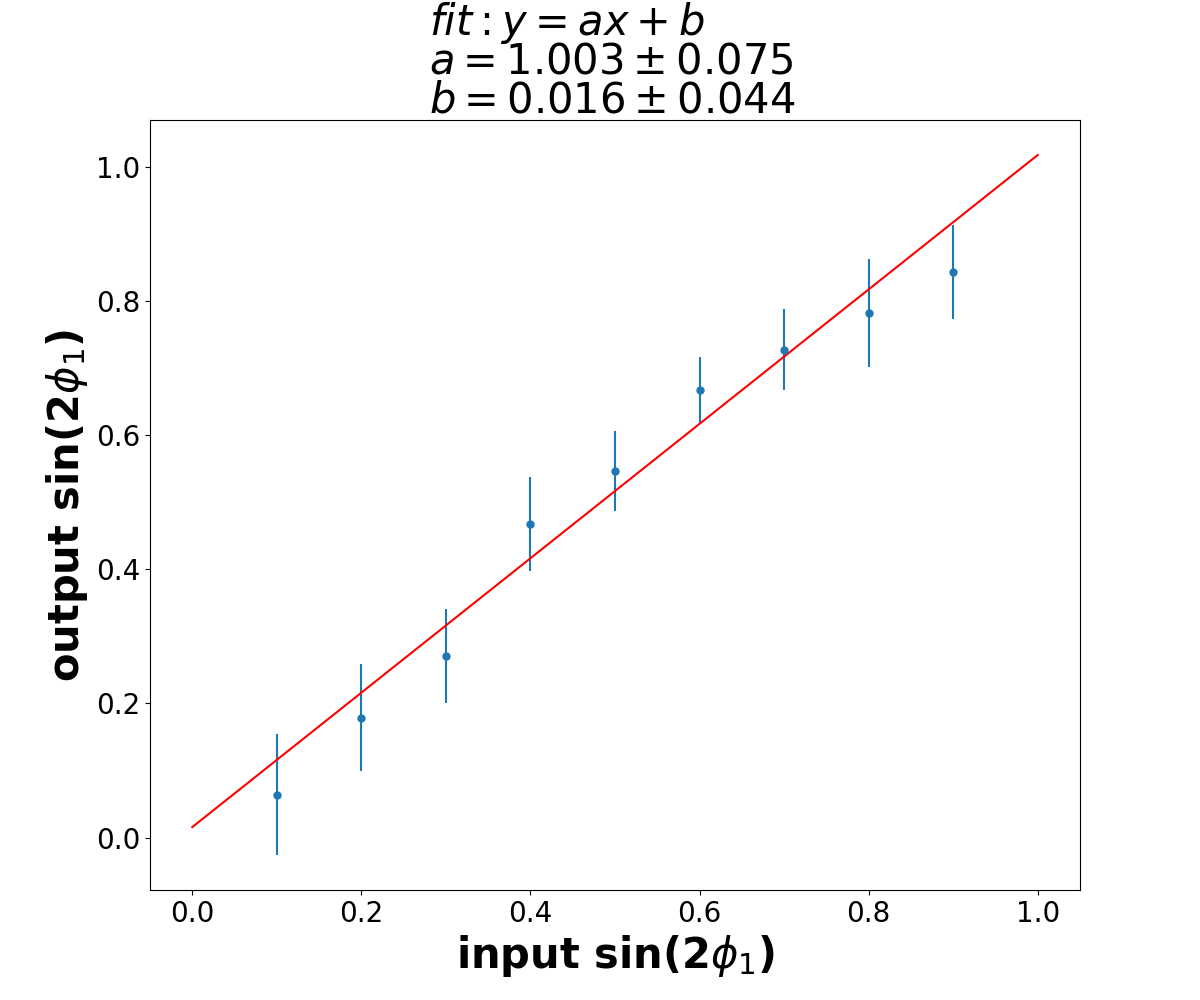
\includegraphics[width=1\linewidth]{figures/S-test-line}
		%\caption{$\it{CP}$ fit on 8873 signal MC.}
	\end{minipage}
	\begin{minipage}{0.5\linewidth}
		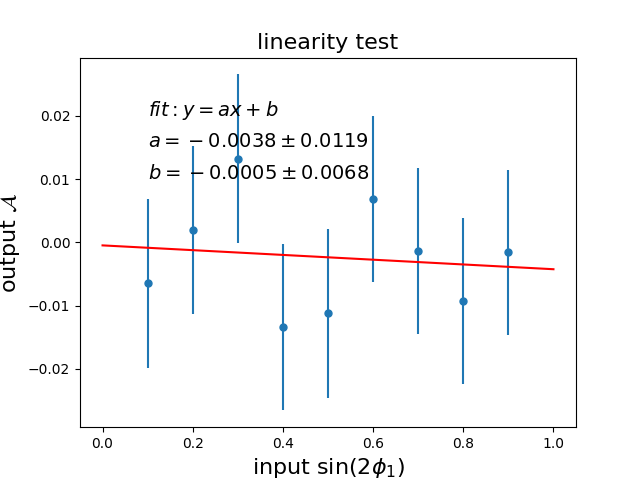
\includegraphics[width=1\linewidth]{figures/A-test-line}
		%\caption{$\it{CP}$ fit on 373 generic MC.}
	\end{minipage}
	\caption{Linearity test of $\it{CP}$ fit with a fixed input $\mathcal{A}=0$ and floating sin$(2\phi_1)$. The left is for the output sin$(2\phi_1)$ and the right is for the output $\mathcal{A}$.}
	\label{fig:cpfit_line_S}
\end{figure}
We fix sin$(2\phi_1)$ at zero while floating $\mathcal{A}$ from  0.1 to 0.9 to repeat the above linearity test. The dependence between input and output are shown in Figure \ref{fig:cpfit_line_A}, where a linear function is used to fit the dependence. 
\begin{figure}[htpb]
	\begin{minipage}{0.5\linewidth}
		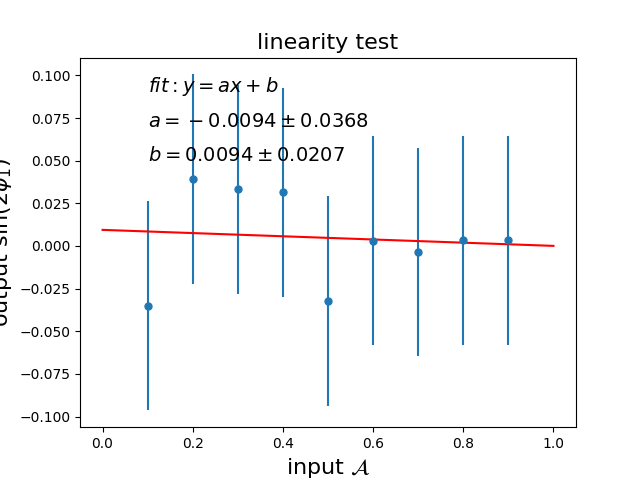
\includegraphics[height=6cm]{figures/S-test-line_fixS}
		%\caption{$\it{CP}$ fit on 8873 signal MC.}
	\end{minipage}
	\begin{minipage}{0.5\linewidth}
		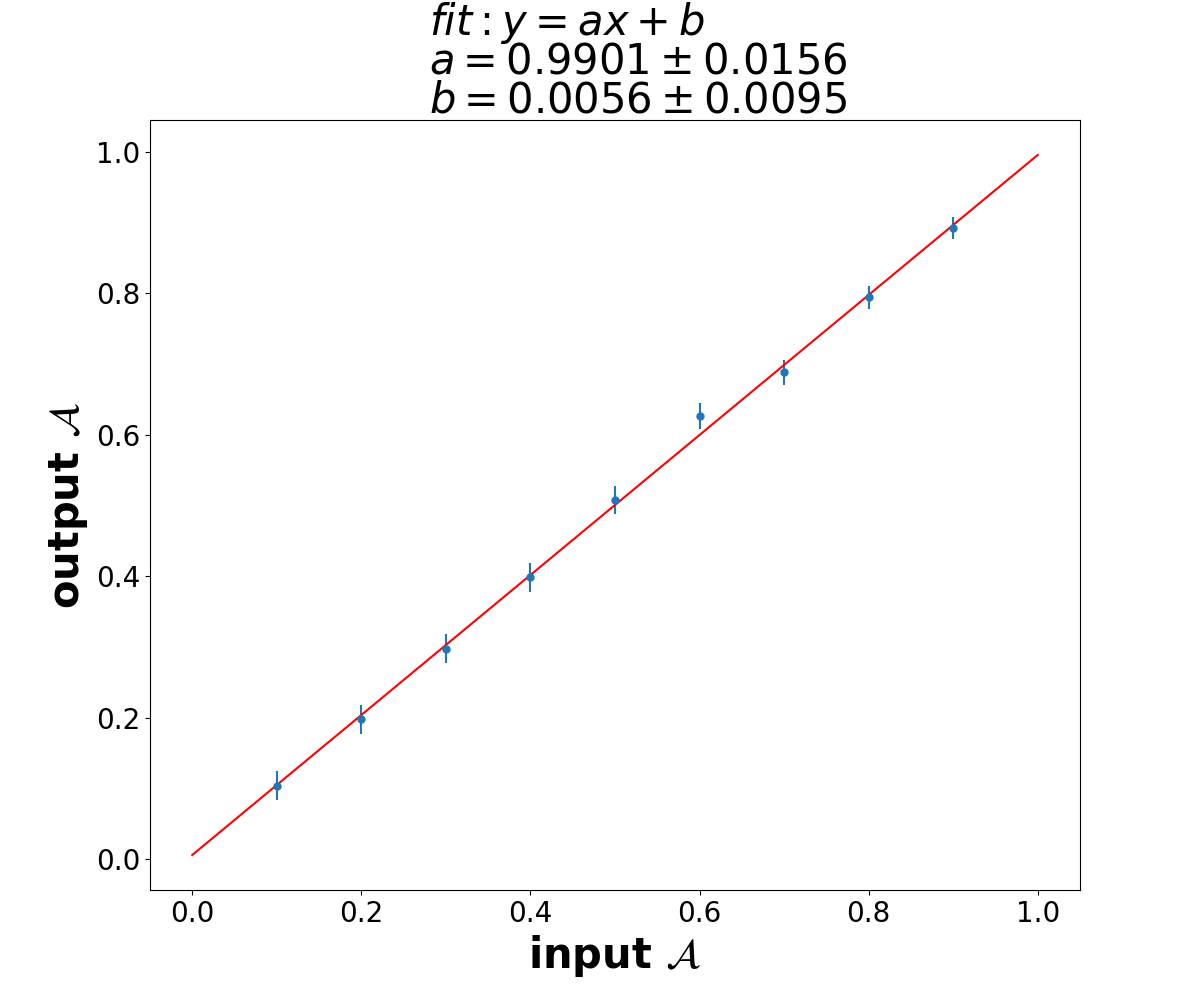
\includegraphics[height=6cm]{figures/A-test-line_fixS}
		%\caption{$\it{CP}$ fit on 373 generic MC.}
	\end{minipage}
	\caption{Linearity test of $\it{CP}$ fit with a fixed input sin$(2\phi_1)=0$ and floating $\mathcal{A}$. The left is for the output sin$(2\phi_1)$ and the right is for the output $\mathcal{A}$.}
	\label{fig:cpfit_line_A}
\end{figure}
From the linear function fit results, the linearity tests show an agreement with the input $\it{CP}$ parameters and the output values. 
\subsection{Toy MC Fit Pull}
In order to check the fit bias and the size of fitted errors with input-output method, a set of 1000 toy MC samples has been created. Each toy MC sample contains 26 events to keep the same number of events as the real data. The $\chi^2$ from vertex fit, the number of events $N$ and vertex errors on $\it{CP}$- and tag-sides are sampled from the distribution of data. The input sin(2$\phi_1$) and $\mathcal{A}$ are both zero for the toy sets. We expect to use the standard normal distribution to fit the pull of sin(2$\phi_1$) and $\mathcal{A}$. 

\begin{figure}[htpb]
	\begin{minipage}{0.5\linewidth}
		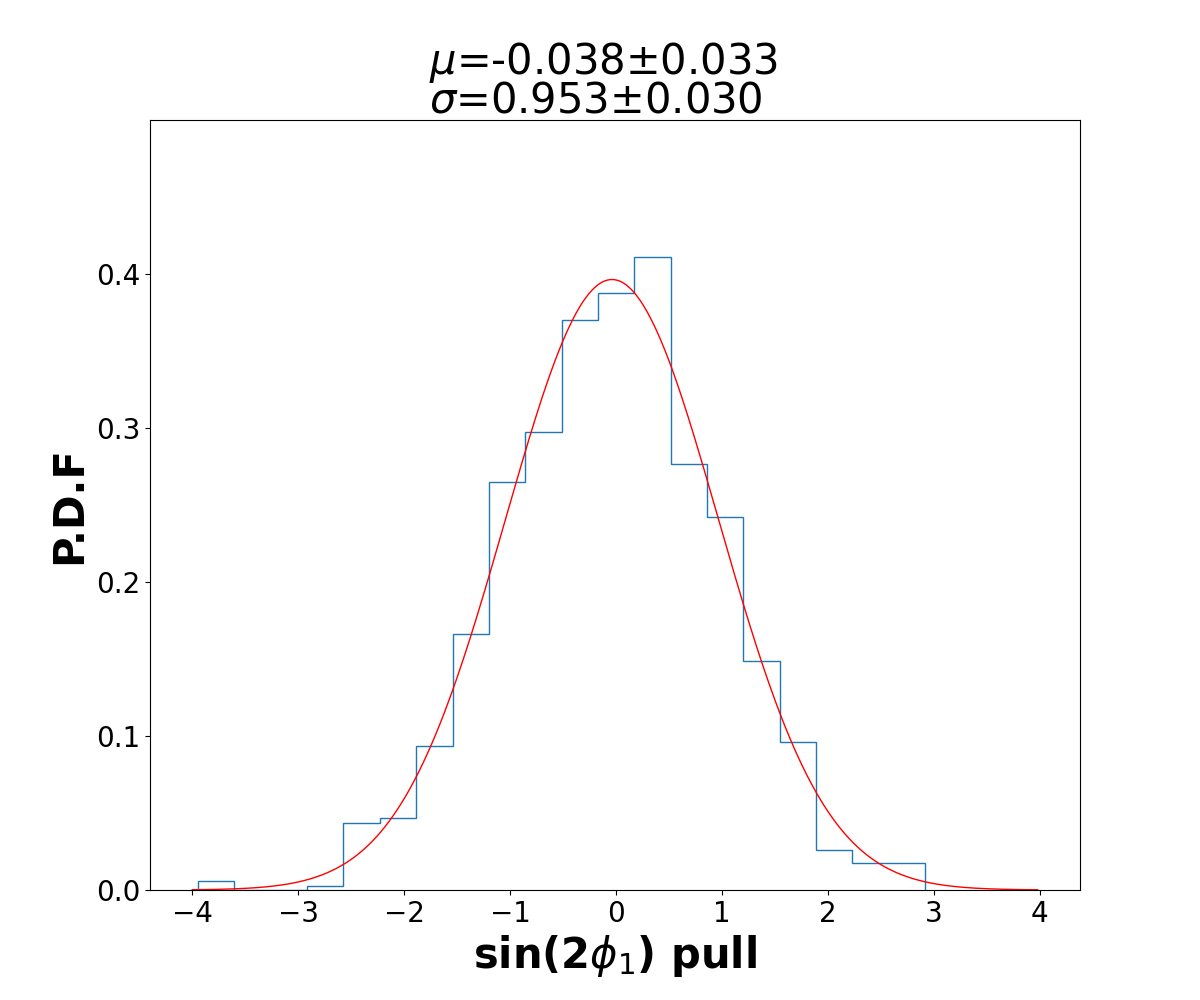
\includegraphics[height=6cm]{figures/pull_hist_S}
		%\caption{$\it{CP}$ fit on 8873 signal MC.}
	\end{minipage}
	\begin{minipage}{0.5\linewidth}
		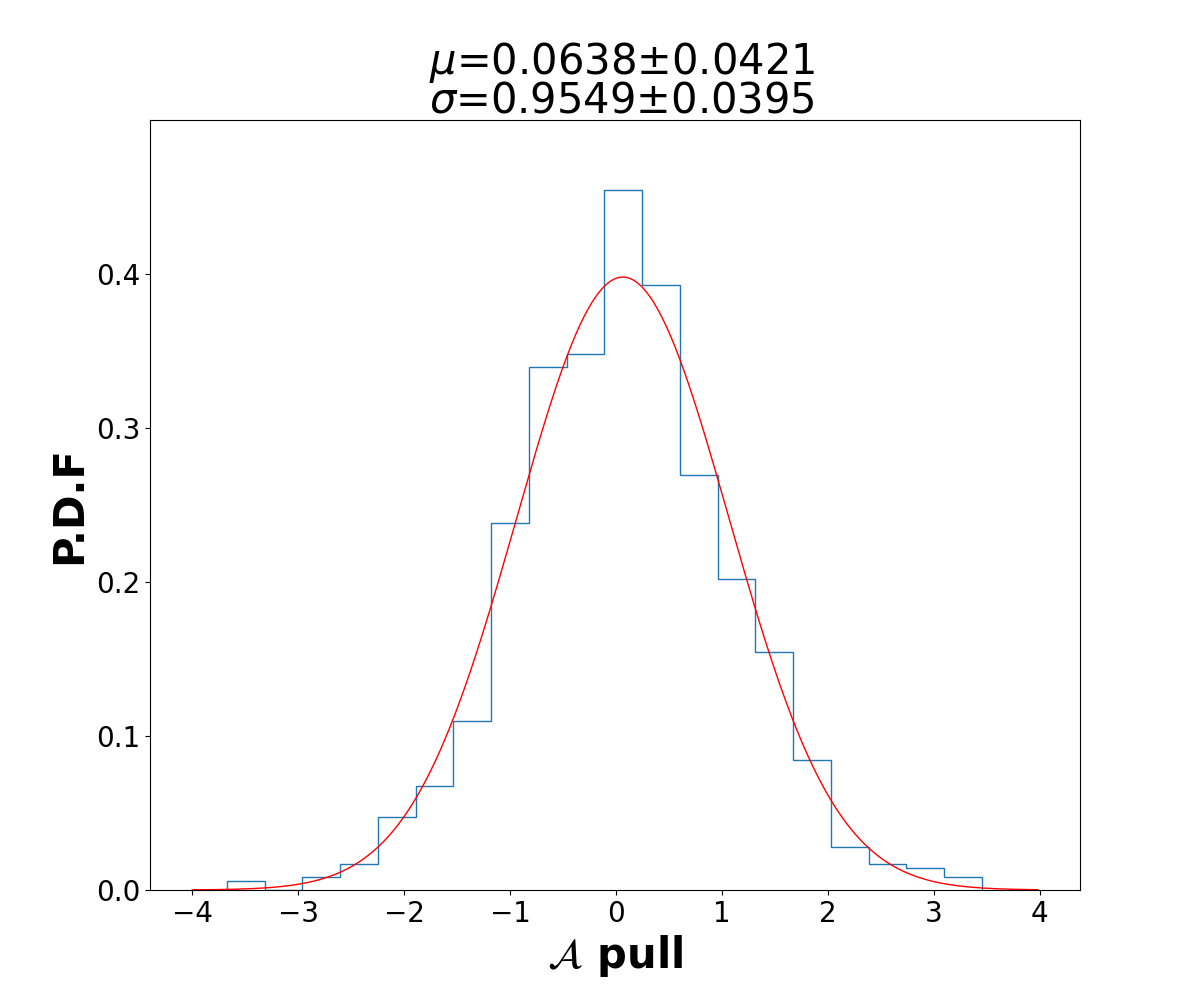
\includegraphics[height=6cm]{figures/pull_hist_A}
		%\caption{$\it{CP}$ fit on 373 generic MC.}
	\end{minipage}
	\caption{The pull distributions of sin$(2\phi_1)$ and $\mathcal{A}$ fitted by the standard normal distribution with $\mu$ as the mean and $\sigma$ as the standard deviation. }\label{fig:pull}
\end{figure}

As shown in Figure \ref{fig:pull}, the fit results using the standard normal distribution shows a good recovery of input sin$(2\phi_1)$ and $\mathcal{A}$ with no clear bias is spotted. The fitted errors look to be a little bit overestimated around 5\% but they are still consistent with 1.5$\sigma$ so that any correction is not applied.


\subsection{Lifetime fit}
Before looking at $\it{CP}$ parameters in data, we need to check if the lifetime of $B$ meson are consistent by configuring the $\it{CP}$ fitter to fit it as a floating parameter. To test lifetime fit, first we use 10000 \textit{signal MC} events which is generated by $\tau_{B^0} = 1.520$ from PDG value. The sin$(2\phi_1)$ and $\mathcal{A}$ are fixed at zero during the fit, for which the generator level $\it{CP}$ violation is zero. This is equivalent fit to Equation \ref{eq:cpfit_mc_life}.
\begin{equation}\label{eq:cpfit_mc_life}
\mathcal{P}(\Delta t,\tau_{B^0}) = 
\frac{e^{-|\Delta t|/\tau_{B^0}}}{4\tau_{B^0}}
\end{equation}
The fit result on \textit{signal MC} is $1.537 \pm 0.024$ ps which is consistent with the input. We perform the lifetime fit on data in signal region, and the $\it{CP}$ parameters are fixed based on PDG values to: sin$(2\phi_1)=0.69$ and $\mathcal{A} = 0$. The fitted lifetime from $B^0 \to K_S^0  K_S^0  K_S^0$ is $1.431\pm 0.382$ ps. The result is consistent with PDG value. The distribution of $\Delta t$ in lifetime fit is shown as Figure \ref{fig:cpfit_data_life}.
The $B^0$ and $B^+$ lifetime fit using control sample is also performed and summarized in Ref.~\cite{jpsiks_ichep}. The results are consistent with PDG values as input in MC generator. 
\begin{figure}[htpb]
	\centering
	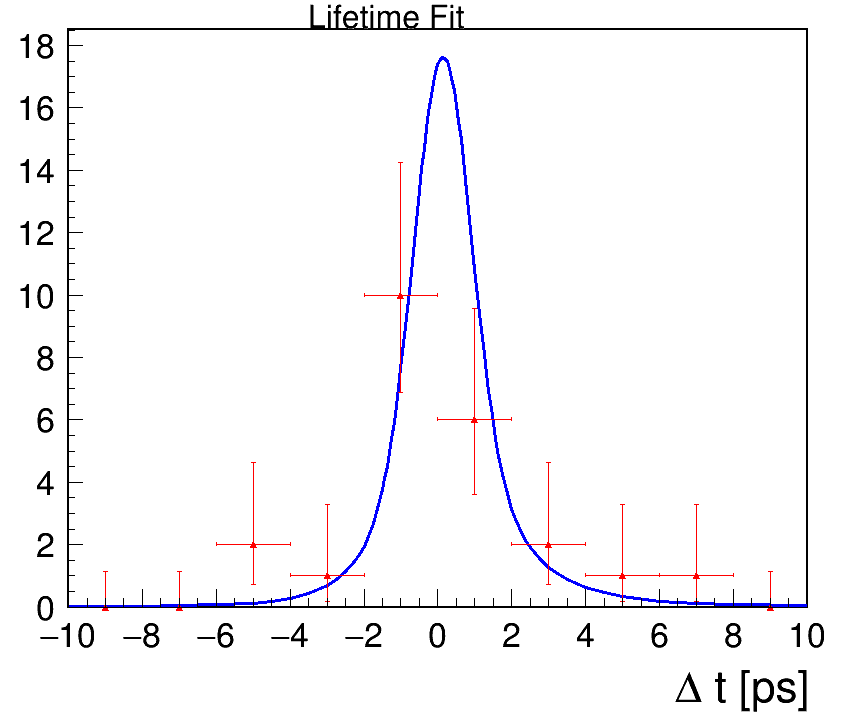
\includegraphics[height=7cm]{figures/lifetime_data}
	\caption{Lifetime fit on data}
	\label{fig:cpfit_data_life}
\end{figure}
%\subsection{Control Sample fit}
\begin{comment}
To test the fit on physics parameter $\Delta m_d$, we generate 200 toy sets with input $\Delta m_d = 0.507 $ GeV/$c^2$ where each set contains 26 events as same as data. The fit result is close to normal distribution and the pull of $\Delta m_d$ is shown in Figure \ref{fig:cpfit_dm_pull}. 
\begin{figure}[htpb]
\centering
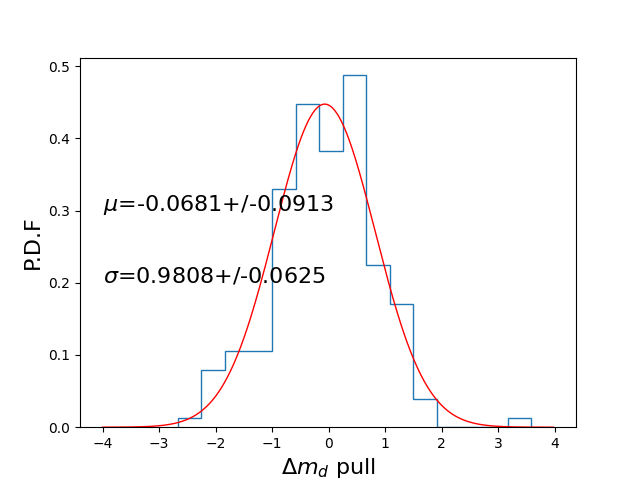
\includegraphics[height=7cm]{figures/pull_hist_dm}
\caption{The pull distribution of $\Delta m_d$ fitted by the standard normal distribution with $\mu$ as the mean and $\sigma$ as the standard deviation. }
\label{fig:cpfit_dm_pull}
\end{figure}
%\subsection{Control Sample fit}
\end{comment}
\section{$\it{CP}$ fit on data}
After the $\it{CP}$ fit procedures are reviewed by Belle II collaboration, the permission of measuring $\it{CP}$ parameters using 62.8 fb$^{-1}$ Belle II data is granted. The events number used for the $\it{CP}$ fit is 26, and the fit result is shown Figure \ref{fig:cpfit_data}.

\begin{figure}[htpb]
	\centering
	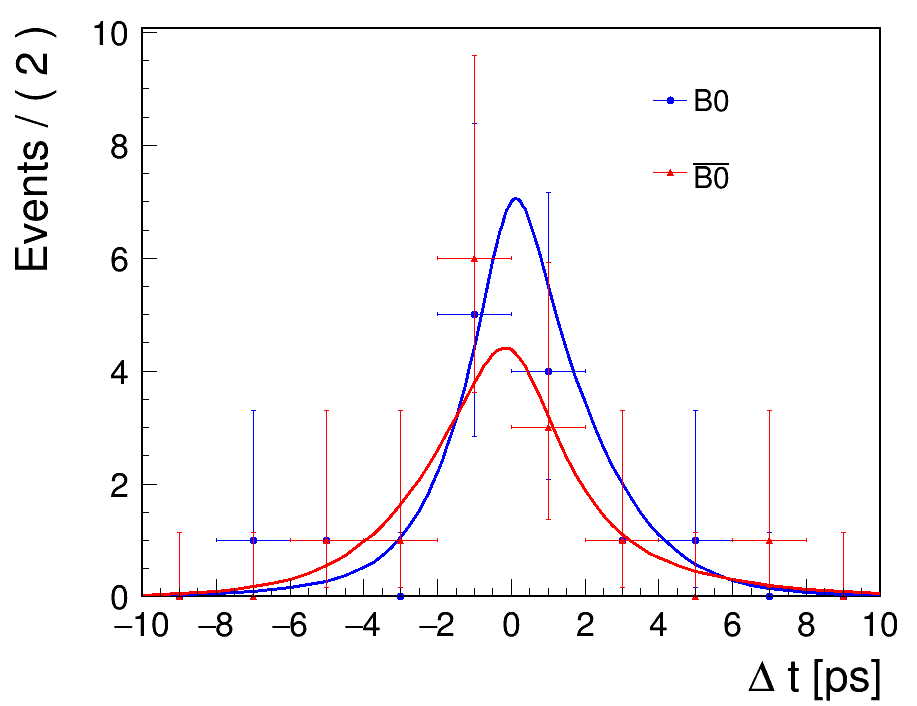
\includegraphics[width=0.7\linewidth]{cpfit-data}
	\caption{The $\it{CP}$ fit result from data. $B^0$ and $\bar{B^0}$ stand for the flavor of the tag-side $B$ meson.}
	\label{fig:cpfit_data}
\end{figure}

The results of $\it{CP}$ parameters are obtained as

\begin{equation}
\begin{split}
sin(2\phi_1) & = 0.82 \pm 0.85~(\text{stat})~, \\
\mathcal{A} & = -0.21 \pm 0.28~(\text{stat})~. \\
\end{split}
\end{equation} 


\section{Systematic Uncertainty}
The systematic uncertainty that affects the $\it{CP}$ fit results may come from many aspects of the measurement procedures. We first estimate the contribution from each source, then the total systematic uncertainty  is calculated by adding-in-quadrature using each contribution. The possible systematic uncertainty from each source is summarized in Table \ref{tab:sy_sub}. 

The contributions from signal and background $\Delta t$ shapes, wrong tag fraction $w$, physics parameters, and signal fraction directly come from the corresponding parameters in the $\it{CP}$ fit model. To be specific, in each above source, if the parameters are defined with MC study, we float the value by $\pm 2 \sigma$, and if the parameters are defined by data, we float the value by $\pm 1 \sigma$, where $\sigma$ is the uncertainty of the parameters. The contribution from every parameter in each source is therefore marked as $\pm \delta \mathcal{S}$ and $\pm \delta \mathcal{A}$, where the signs present the difference caused by positively or negatively floating values. In the case, from Table \ref{tab:sy_sigt} to Table \ref{tab:sy_fsig}, the total $\delta \mathcal{S}$ and  $\delta \mathcal{A}$ are obtained by adding in quadrature using all $\pm \delta \mathcal{S}$ and $\pm\delta \mathcal{A}$, respectively. From Table \ref{tab:fitbias} to Table \ref{tab:sy_vertex}, the total $\delta \mathcal{S}$ and  $\delta \mathcal{A}$ are calculated directly by adding in quadrature of the contribution from every source.

\begin{table}[H]
	\centering
	\caption{The contributions of each source and the total systematic uncertainty.  }
	\label{tab:sy_sub}
	\begin{tabular}{c|r|r} 
		\hline
		Sources &  $\delta \mathcal{S}$ & $\delta \mathcal{A}$\\
		\hline
		signal $\Delta t$ shapes & 0.034 & 0.0093 \\
		background $\Delta t$ shapes & 0.039 & 0.037\\
		wrong tag fraction & 0.0037 & 0.0038\\
		physics parameters & 0.0069 & 0.0013\\ 
		signal fraction  & 0.044 & 0.034 \\
		fit bias & 0.0098 & 0.0057 \\
		\textcolor{black}{\textit{KsFinder} impact on data} & $0.0036$ & $0.0036$\\
		\textcolor{black}{vertex reconstruction} & 0.019 & 0.021\\
		\textcolor{black}{tag-side interference} & 0.001 & 0.008\\
		\hline
		Total & 0.072 & 0.056\\
		\hline
	\end{tabular}
\end{table}

\begin{comment}
\begin{table}[H]
\centering
\caption{The contributions of each source and the total systematic uncertainty.  }
\label{tab:sy_sub}
\begin{tabular}{c|r|r} 
\hline
Sources &  $\delta \mathcal{S}$ & $\delta \mathcal{A}$\\
\hline
signal $\Delta t$ shapes & 0.033793 & 0.009283 \\
background $\Delta t$ shapes & 0.039430 & 0.037269\\
wrong tag fraction & 0.003709 & 0.003790\\
physics parameters & 0.006923 & 0.001250\\ 
signal fraction  & 0.044387 & 0.033932 \\
fit bias & 0.009817 & 0.005702 \\
\textit{KsFinder} impact on data & $0.003640$ & $0.003584$\\
vertex reconstruction & 0.019007 & 0.020563\\
tag-side interference & 0.001000 & 0.008000\\
\hline
Total & 0.072114 & 0.056344\\
\hline
\end{tabular}
\end{table}
\end{comment}

On the other hand, for the contributions from fit bias, \textit{KsFinder}, and vertex reconstruction, they are not directly from the parameters of the fit model, but the number of events in fit bias test, \textit{KsFinder} correction factor, and vertex reconstruction options, respectively. We modify their values or ranges to repeat the $\it{CP}$ fit to obtain their contributions as $\delta \mathcal{S}$ and $\delta \mathcal{A}$ correspondingly. 

Last but not least, tag-side interference could also contribute to the total systematic uncertainty, which is caused by the interference between CKM-favored or CKM-suppressed tree-level decays.  There is no estimation on systematic uncertainty from the tag-side interference in the Belle II at the current stage. Since this effect is less sensitive to the detector performance, we quote the value from the Belle $\delta \mathcal{S} \sim 0.001$ and $\delta \mathcal{A} \sim 0.008$~\cite{yosuke2011measurement},  which is a small contribution compared to the current statistical uncertainty.

In the following sections, the estimations of systematic uncertainty from each source in Table \ref{tab:sy_sub} are discussed in detail.
\begin{comment}
\begin{itemize}
\item resolution functions parameters
\item signal fraction
\item flavor tagging 
\item background $\Delta t$ shapes
\item fit bias
\item physics parameters
\item KsFinder impact on data
\item vertex reconstruction
\end{itemize}
\end{comment}

\subsection{Systematic uncertainty from signal $\Delta t$ shapes}
The signal $\Delta t$ shapes are dependent on the resolution functions of $\it{CP}$- and tag-sides, therefore the contributions come from the parameters used in the corresponding models, which are determined by using MC samples. The contributions from each parameters are summarized in Table \ref{tab:sy_sigt}, which are obtained by floating $2\sigma$ for each of them.

\begin{table}[htpb]
\begin{minipage}[b]{1.0\linewidth}
\centering
\caption{Systematic uncertainty from signal $\Delta t$ shapes}
\label{tab:sy_sigt}
\begin{tabular}{c r r r r}
\hline
source & $+\delta \mathcal{S}$ & $+\delta \mathcal{A}$ & $-\delta \mathcal{S}$ &  $-\delta \mathcal{A}$\\
\hline
$f_{cp}^{tail}$ & -0.000096 & -0.000057
& 0.000014
& 0.000056
\\
$s_{0CP}^{main}$& 0.0054
& 0.0013
& -0.0057
& -0.0014
\\
$s_{1CP}^{main}$ & 0.020
& -0.00090
& -0.020
& 0.00063
\\
$s_{0CP}^{tail}$ &  -0.0032
& -0.0016
& 0.0033
& 0.0016
\\
$s_{1CP}^{tail}$ & -0.0020	
&-0.000063	
&0.0020	
&0.000048
\\
$f_{tag}^{tail}$ & 0.0031
& -0.0013
& -0.0031
& 0.0013
\\
$s_{0tag}^{main}$&  0.0020
& -0.0014
& -0.0020
& 0.0014
\\
$s_{1tag}^{main}$ & 0.0051
& -0.00084
& -0.0050
& 0.00083
\\
$s_{0tag}^{tail}$ &  -0.00014
& -0.00039
& 0.00010 & 0.00044
\\
$s_{1tag}^{tail}$  & 0.00010& 0.000027 &  -0.00047
& 0.00013
\\
$f_{\delta}$ & -0.0072
& -0.00055
& 0.0072
& 0.00059
\\
$f_p$ &  0.0030
& 0.0043
& -0.0031
& -0.0043
\\
$\tau_n$ & -0.0010 & -0.0028
& 0.00094
& 0.0029
\\
$\tau_p$ &  0.0045
& 0.0025
& -0.0046
& -0.0025
\\
\hline
Total &
\multicolumn{2}{c}{$\delta \mathcal{S}=0.034$} &
\multicolumn{2}{c}{$\delta \mathcal{A}=0.0093$}\\
\hline
\end{tabular}
\end{minipage}
\end{table}

\subsection{Systematic uncertainty from background $\Delta t$ shapes}
The background $\Delta t$ shapes are affected by the resolution model for background events which are
determined by using the sideband data $M_{bc}<5.26$ GeV. In this case, we float $1\sigma$ for each parameter and the results are summarized in Table \ref{tab:sy_bkgt}.

\begin{table}[htpb]
\begin{minipage}[b]{1.0\linewidth}
\centering
\caption{Systematic uncertainty from background $\Delta t$ shapes}
\label{tab:sy_bkgt}
\begin{tabular}{c r r r r}
\hline
source & $+\delta \mathcal{S}$ & $+\delta \mathcal{A}$ & $-\delta \mathcal{S}$ &  $-\delta \mathcal{A}$\\
\hline
$\mu^{bkg}_{\delta}$ & -0.014
& -0.017
& 0.0068
& 0.0065
\\
$\mu^{bkg}_{l}$&  -0.0028
& -0.013
& 0.0038
& 0.013
\\
$\tau_{bkg}$ & 0.0014
& 0.0017
& -0.0042
& 0.000085\\
$f_{\delta}^{bkg}$ &  -0.011
& 0.0014
& 0.011
& -0.0014
\\
$f^{bkg}_{tail}$  &-0.0027
& 0.0015
& 0.0025
& -0.0014
\\
$\sigma^{bkg}_{main}$ & 0.021
& 0.022
& -0.024
& -0.016
\\
$\sigma^{bkg}_{tail}$ & -0.00028 & -0.00016
& 0.00018
& 0.00014
\\
\hline
Total &
\multicolumn{2}{c}{$\delta \mathcal{S}=0.039$} &
\multicolumn{2}{c}{$\delta \mathcal{A}=0.037$}\\
\hline
\end{tabular}
\end{minipage}
\end{table}



\subsection{Systematic uncertainty from wrong tag fraction}
The wrong tag fraction for each event during the $\it{CP}$ fit is obtained by calculating the fraction of wrongly tagged events in the corresponding $r$-bin. As discussed in section 5.2, there are totally seven $r$-bins, marked as $w_1 \sim w_7$. We use the values of $w$ obtained by the tagging control sample study~\cite{abudinen2020first} and float $1\sigma$ to get the contributions. The results are shown in Table \ref{tab:sy_wtag}.


\begin{table}[htpb]
\begin{minipage}[b]{1.0\linewidth}
\centering
\caption{Systematic uncertainty from wrong tagging fraction}
\label{tab:sy_wtag}
\begin{tabular}{c r r r r}
\hline
source & $+\delta \mathcal{S}$ & $+\delta \mathcal{A}$ & $-\delta \mathcal{S}$ &  $-\delta \mathcal{A}$\\
\hline
$w_1$ & -0.0019
& 0.0019
& 0.0019
& -0.0020
\\
$ w_2$ & -0.0016
& 0.0011
& 0.0016
& -0.0012
\\
$ w_3$ & -0.00049
& 0.0013
& 0.00047
& -0.0013
\\
$ w_4$ & 0.00066
& 0.00026
& -0.00065
& -0.00026\\
$ w_5$ & -0.00012
& 0.00020
& 0.00012 &
-0.00020
\\
$ w_6$ & 0.000095 & 0.000054 & 0.000096 & -0.000045 \\
$ w_7$ & 0.00019
& -0.00040
& -0.00019
& 0.00040
\\
\hline
Total &
\multicolumn{2}{c}{$\delta \mathcal{S}=0.0037$} &
\multicolumn{2}{c}{$\delta \mathcal{A}=0.0038$}\\
\hline
\end{tabular}
\end{minipage}
\end{table}


\subsection{Systematic uncertainty from physics parameters.}
The physics parameters that affect the $\it{CP}$ fit are the lifetime of $B^0$ ($\tau_{B^0}$) and the mass difference of the two mass eigenstates of neutral $B$ meson ($\Delta M_d$), which are set as constants in the $\it{CP}$ fit based on the PDG value.
Thus, the contributions from $\Delta m_d$ and $\tau_{B^0}$ are included by floating $1\sigma$ using the PDG average errors. The results are summarized in Table \ref{tab:sy_phys}.
\begin{table}[htpb]
	\begin{minipage}[b]{1.0\linewidth}
		\centering
		\caption{Systematic uncertainty from  physics parameters}
		\label{tab:sy_phys}
		\begin{tabular}{c r r r r}
			\hline
			source & $+\delta \mathcal{S}$ & $+\delta \mathcal{A}$ & $-\delta \mathcal{S}$ &  $-\delta \mathcal{A}$\\
			\hline
			$\Delta m_d$  & -0.0018
			& -0.00069
			& 0.0018
			& 0.00070
			\\
			$\tau_{B^0}$  & -0.0046
			& -0.00055
			& 0.0046
			& 0.00056
			\\
			\hline
			Total &
			\multicolumn{2}{c}{$\delta \mathcal{S}=0.0069$} &
			\multicolumn{2}{c}{$\delta \mathcal{A}=0.0013$}\\
			\hline
		\end{tabular}
	\end{minipage}
\end{table}


\subsection{Systematic uncertainty from signal fraction.}
The signal fraction is a event-by-event parameter based on the $M_{bc}$ and $\Delta E$ which is determined using 2D fit results from data. Because of this, we take turns to change each parameter in the 2D fit by floating $1\sigma$ to get different 2D fit models. Then based on each model, signal fraction parameter for every event is updated and used during the $\it{CP}$ fit. The $M_{bc}$ and $\Delta E$ models are single and triple Gaussian functions, thus there are 8 parameters for the means and standard deviations, as well as 2 internal fraction coefficients for the triple Gaussian functions of $\Delta E$. Besides the shape parameters in each model, the signal fraction is the floating parameter to be obtained by the 2D fit. We also directly float the signal fraction by $1\sigma$ to check its contribution. 
The results are summarized in Table \ref{tab:sy_fsig}.
\begin{table}[htpb]
	\begin{minipage}[b]{1.0\linewidth}
		\centering
		\caption{Systematic uncertainty from  signal fraction}
		\label{tab:sy_fsig}
		\begin{tabular}{c r r r r}
			\hline
			source & $+\delta \mathcal{S}$ & $+\delta \mathcal{A}$ & $-\delta \mathcal{S}$ &  $-\delta \mathcal{A}$\\
			\hline
			$\mu_{mbc}$  & 0.00082 &	-0.0039&	-0.00080&	0.0038
			\\
			$\sigma_{mbc}$ & 0.00048 &	0.0084&	-0.00063&	-0.0087
			\\
			$\chi_{argus}$ & -0.00071&	0.0041	&0.0014&	-0.0058
			\\
			$c_{argus}$ & -0.0055&	0.0014&	0.0009&	-0.000078\\
			$f^1_{\Delta E}$ & 0.028 &	0.021&	-0.019	&-0.0084
			\\
			$f^2_{\Delta E}$ & 0.021&	0.018	&-0.016	&-0.0070
			\\
			$\mu^1_{\Delta E}$ & -0.00044&	-0.00015&	0.00050&	0.000088\\
				$\mu^2_{\Delta E}$& -0.00056&	0.0014&	0.00059&	-0.0014
			\\
				$\mu^3_{\Delta E}$ & -0.0032&	-0.00083&	0.0034&	0.00098
			\\
				$\sigma^1_{\Delta E}$& -0.00017&	-0.00097&	0.00021&	0.00091
			\\
			$\sigma^2_{\Delta E}$& -0.0032&	0.0030&	0.0026&	-0.0025
			\\
			$\sigma^3_{\Delta E}$& -0.0019&	-0.0026&	0.0025&	0.0030
			\\
			$a_{cheb}$ & 0.00095&	0.000057&	-0.00089&	-0.00010
			\\
			$f_{sig}$ & -0.0046&	0.0040&	0.0049&	-0.0035
			\\
			\hline
			Total &
			\multicolumn{2}{c}{$\delta \mathcal{S}=0.044$} &
			\multicolumn{2}{c}{$\delta \mathcal{A}=0.034$}\\
			\hline
		\end{tabular}
	\end{minipage}
\end{table}


\subsection{Systematic uncertainty from fit bias.}
Using maximum likelihood fit might cause bias to the fit results, which can be checked by using a large number of input events. We use 300000 \textit{signal MC}  events with zero $\it{CP}$ violation to evaluate such effect. The fit result is $\mathcal{S} = 0.000127\pm0.009817$ and $\mathcal{A} = 0.000265\pm0.005702$. The difference between the output of the $\it{CP}$ fit and input ($\mathcal{S}=0$) for $\mathcal{S}$ is 0.000127 and the fit error is 0.009817, and we use the larger one among them as the fit bias contribution, as listed in Table \ref{tab:fitbias}.

\begin{table}[htpb]
	\begin{minipage}[b]{1.0\linewidth}
		\centering
		\caption{Systematic uncertainty from fit bias}
		\label{tab:fitbias}
		\begin{tabular}{c r r}
			\hline
			source & $\delta \mathcal{S}$ & $\delta \mathcal{A}$ \\
			\hline
			fit bias & 0.0098 & 0.0057\\
			\hline
		\end{tabular}
	\end{minipage}
\end{table}


\subsection{Systematic uncertainty from \textit{KsFinder}.}
Applying \textit{KsFinder} cut at 0.74 based on MC study may introduce small bias on data due to the different response on the classifier between data and MC. Therefore the systematic uncertainty from applying \textit{KsFinder} is considered. As discussed in section 3.2.7, the upper and lower limit of  $\mathcal{R}_{B^0}$ are 1.033 and 0.967 respectively. These two ratios are applied on the data events obtained  to repeat the $\it{CP}$ fit, and the difference of fit results compared to the original values are used as systematic uncertainties, as shown in Table \ref{tab:sy_ks}.

\begin{table}[htpb]
	\begin{minipage}[b]{1.0\linewidth}
		\centering
		\caption{Systematic uncertainty from \textit{KsFinder}.}
		\label{tab:sy_ks}
		\begin{tabular}{c r r}
			\hline
			source & $\delta \mathcal{S}$ & $\delta \mathcal{A}$ \\
			\hline
			$\mathcal{R}_{B^0}=1.033$ & 0.0025
 & -0.0025\\
			$\mathcal{R}_{B^0}=0.967$ & -0.0026
& 0.0026
\\
			\hline
			Total &
			{$0.0036$} &
			{$0.0036$}\\
			\hline
		\end{tabular}
	\end{minipage}
\end{table}

\subsection{Systematic uncertainty from vertex reconstruction.}
For vertex reconstruction, the contributions from the options in Table \ref{tab:cutCP} are considered. Given the fact that cut values in Table \ref{tab:cutCP} are very loose and the number of events from data is very limited, the changing of the these values does not affect events collected from data so that systematic uncertainty can not be reflected correctly. Therefore, 1 ab$^{-1}$ \textit{generic MC} is used with the modified ranges to estimate the potential systematic uncertainty from vertex reconstruction. Besides, due to the absence of IP constraint in vertex fit, the contributions from the IP constraint options as well as the potential bias are not considered. However, this does not mean that the IP constraint options have no effect on the $\it{CP}$ fit. Since we also do not use any IP constraint options in the study of the vertex resolution functions, the resolution observed in this case will be worse compared to the ones with good IP constraint and tighter vertex selection criteria. Thus, the systematic uncertainties from $\Delta t$ shapes become larger, already indirectly reflecting the contributions from the missing IP options. Besides, the contributions due to the VXD misalignment and $\Delta z$ bias are not included because the PXD is not fully installed and the beam misalignment is not well understood in the early stage of the Belle II.
The results are listed in Table \ref{tab:sy_vertex}, where the zero values appear due to the unchanged events input under the modified ranges. This part of the systematic uncertainty will be checked with more data and \textit{generic MC} in future to testify the possible variation.

\begin{table}[htpb]
	\begin{minipage}[b]{1.0\linewidth}
		\centering
		\caption{Systematic uncertainty from vertex reconstruction}
		\label{tab:sy_vertex}
		\begin{tabular}{c r r}
			\hline
			source & $\delta \mathcal{S}$ & $\delta \mathcal{A}$ \\
			\hline
			$\sigma_{z_{tag}}<0.05$ cm & 0.0044
& -0.0036
\\
			$\sigma_{z_{tag}}<0.15$ cm & 0.00 & 0.00 \\
			$\chi^2/N(CP)<3$ & 0.018
& -0.020
\\
			$\chi^2/N(CP)<13$ & 0.00 & 0.00\\
			$\chi^2/N(tag)<40$ & 0.00
& 0.00
\\
			$\chi^2/N(tag)<60$ & 0.00 & 0.00\\
			$|\Delta t|<50 $ ps & 0.0033
& -0.00040
\\
			$|\Delta t|<90 $ ps & 0.00 & 0.00\\
			IP constraint & 0.00& 0.00\\
						\hline
							Total &
						{$0.019$} &
						{$0.021$}\\
\hline
		\end{tabular}
	\end{minipage}
\end{table}

In conclusion, the current systematic uncertainty is estimated by considering each possible source, where the total systematic uncertainty of $\delta \mathcal{S}_{syst} \simeq 0.07$ and $\delta \mathcal{A}_{syst} \simeq 0.06$ are obtained. It is clear that the dominated uncertainty at the current stage of the Belle II for time-dependent $\it{CP}$ violation measurement in $B^0 \to K_S^0  K_S^0  K_S^0$ is still the statistical error. As a result, the 
current results are agreed with the previous results from Belle, as well as the SM predictions.

However, this might be changed in future when more data becomes available. In the meantime, some of the systematic uncertainty sources are considered as the reducible contributions while the others remain almost unchanged with increasing mount of data and MC samples. The prospective of the statistical and systematic uncertainties in future are fundamentally important to examine the SM predictions and search for the NP effects in this decay mode. We will discuss about the future statistical and systematic uncertainties of $\mathcal{S}$ in detail in the next chapter.


